\documentclass{article}

% Language setting
% Replace `english' with e.g. `spanish' to change the document language
\usepackage[english]{babel}

% Set page size and margins
% Replace `letterpaper' with`a4paper' for UK/EU standard size
\usepackage[letterpaper,top=2cm,bottom=2cm,left=3cm,right=3cm,marginparwidth=1.75cm]{geometry}

% Useful packages
\usepackage{amsmath}
\usepackage{graphicx}
\usepackage{subfig}

\usepackage{multicol}
\usepackage{placeins}

\usepackage[colorlinks=true, allcolors=blue]{hyperref}

\graphicspath{ {./figures/} }

\title{Student Performance Analysis and Prediction \\ Final project for the Foundations of Data Science course \\(a.a. 2023/2024) }
\author{Paolo Cursi 2155622, Tommaso Leonardi 1914546, \\Arianna Paolini 1943164, Stefano Saravalle 1948684, Pietro Signorino 2149741}

\begin{document}
\maketitle

\begin{abstract}
Academic success is relevant to students satisfaction and consequent commitment in studying, leading them to become well formed professional figures. This project aims to understand which are the factors that influence the most the scores that the students get in their exams, by considering the case of the British Open University. Linear and non-linear machine learning models have been trained to predict the performance of the students in various assessments.
\end{abstract}

\section{Introduction}
The Open University is a public university in England that provides data about demographic information and academic performance of its students in order to allow learning analytics. We based our project on \textit{The Open University Learning Analytics dataset}, which is also available on Kaggle (\url{https://www.kaggle.com/datasets/rocki37/open-university-learning-analytics-dataset}). \\

We were interested in this dataset as it provides data about students interaction with the \textit{Virtual Learning Environmment} (\textit{VLE}), an online platform holding teaching materials and resources for the university courses. This could be an opportunity to test how much new technologies can help the learning process. That, combined with the availability of information about the social status of the students (age, gender, disability, education level, etc.) and their academic career (scores in assessment, number of studied credits, etc.) makes the Open University dataset a good choice for our purposes. \\

We selected different machine learning models to implement the prediction of students scores in assessments, both in the form of a regression and a multinomial classification task (by dividing the students according to some thresholds on the score range): \textit{linear regression}, \textit{decision trees} and \textit{KNN regression} will be used for regression, \textit{logistic regression }and \textit{neural networks} for classification. Having multiple trained models for each task allows us to compare the results we get, to determine which model performs best and to try to understand why so. The code of our work can be found at \url{https://github.com/twgever/FDS_Project}. %rendere pubblica

\section{Dataset}

\begin{figure}[h!]
\centering
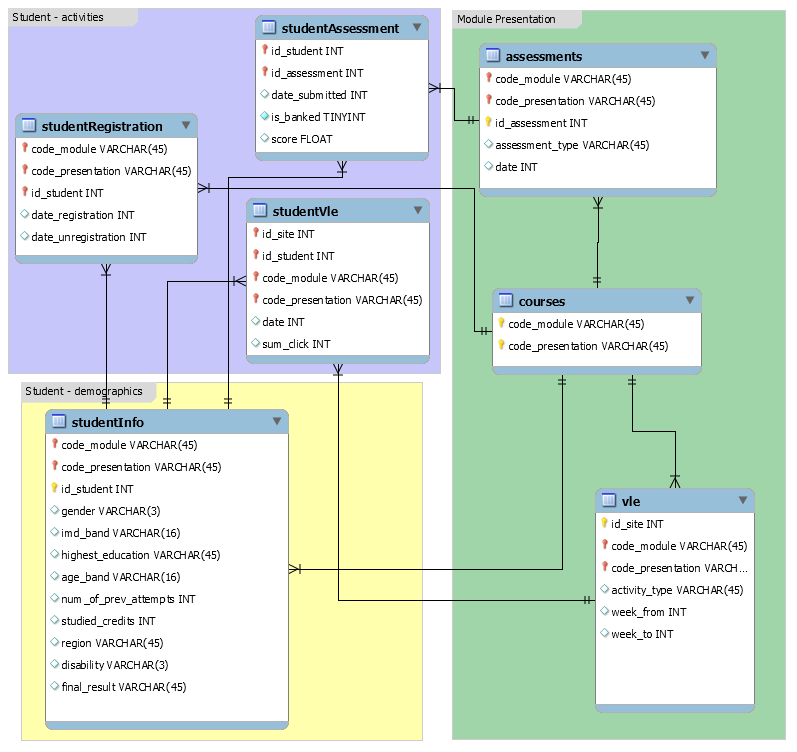
\includegraphics[width=0.7\textwidth]{database.png}
\caption{\label{fig:dataset}The organization of the tables in the Open University Learning Analytics dataset (\url{https://analyse.kmi.open.ac.uk/open_dataset})}
\end{figure}

The Open University Learning Analytics dataset contains data about 22 courses with 32,593 registered students \cite{dataset}. It is organized in seven relational tables, as shown in Figure \ref{fig:dataset}:
\begin{itemize}
    \item \textbf{courses}: includes the list of all available courses (which are called \textit{modules}) and their \textit{presentations} (i.e. the occurence of a course in a specific academic year). The columns are:
    \begin{itemize}
        \item \textit{code module}: code name of the module, which serves as the identifier;
        \item \textit{code presentation}: code name of the presentation, which consists of the year and “B” for the presentation starting in February or “J” for the presentation starting in October;
        \item \textit{length}: length of the module-presentation in days.
    \end{itemize}

    \item \textbf{assessments}: contains information about assessments in module-presentations, which are typically a number of assessments followed by the final exam. The columns are:
    \begin{itemize}
        \item \textit{code module}: identification code of the module to which the assessment belongs;
        \item \textit{code presentation}: identification code of the presentation to which the assessment belongs;
        \item \textit{id assessment}: identification number of the assessment;
        \item \textit{assessment type}: type of assessment, it can be: Tutor Marked Assessment (TMA), Computer Marked Assessment (CMA) or Final Exam (Exam);
        \item \textit{date}: information about the final submission date of the assessment calculated as the number of days since the start of the module-presentation (the starting date of the presentation has number 0);
        \item \textit{weight}: weight of the assessment in percentage; final exams are treated separately and have weight 100\%, the sum of all other assessments is 100\%.  
    \end{itemize}
    
    
    \item \textbf{vle}: includes data about the available materials in the VLE (html pages, pdf files, etc.); students interactions with the materials are recorded. The table contains the following columns:
    \begin{itemize}
        \item \textit{id site}: an identification number of the material;
        \item \textit{code module }: an identification code for the module;
        \item \textit{code presentation}: an identification code of the presentation;
        \item \textit{activity type}: the role associated with the module material;
        \item \textit{week from}: the week from which the material is planned to be used;
        \item \textit{week to}: week until which the material is planned to be used.
    \end{itemize}

    \item \textbf{studentInfo}: contains demographic information about the students attending each of the modules, together with their results. The columns are:
    \begin{itemize}
        \item \textit{code module}: an identification code for a module on which the student is registered;
        \item \textit{code presentation}: the identification code of the presentation during which the student is registered on the module;
        \item \textit{id student}: a unique identification number for the student;
        \item \textit{gender}: the student’s gender;
        \item \textit{region}: identifies the geographic region, where the student lived while taking the module-presentation;
        \item \textit{highest education}: highest student education level on entry to the module-presentation;
        \item \textit{imd band}: specifies the \textit{Index of Multiple Depravation band} of the place where the student lived during the module-presentation;
        \item \textit{age band}: band of the student’s age;
        \item \textit{num. of prev. attempts }: the number of times the student has attempted this module;
        \item \textit{studied credits}: the total number of credits for the module the student is currently studying;
        \item \textit{disability}: indicates whether the student has declared a disability;
        \item \textit{final result}: student’s final result in the module-presentation.
    \end{itemize}

    \item \textbf{studentRegistration}: contains information about the time when the student registered or unregistered for the module-presentation. The colums are:
    \begin{itemize}
        \item \textit{code module}: an identification code for the module;
        \item \textit{code presentation}: the identification code of the presentation;
        \item \textit{id student}: a unique identification number for the student;
        \item \textit{date registration}: the date of the student’s registration to the module-presentation, as the number of days measured relative to the start of the module-presentation (e.g. the negative value -30 means that the student registered to module-presentation 30 days before it started);
        \item \textit{date unregistration}: date of student's unregistration from the module-presentation (students  who completed the course have this field empty; students who unregistered have withdrawal as the value of the \textit{final result} column in the \textit{studentInfo} table).
    \end{itemize}

    \item \textbf{studentAssessment}: shows the results of students’ assessments. If the student does not submit the assessment, no result is recorded. The final exam submissions is missing if the result of the assessments is not stored in the system. It contains the following columns:
    \begin{itemize}
        \item \textit{id assessment}: the identification number of the assessment;
        \item \textit{id student}: a unique identification number for the student;
        \item \textit{date submitted}: the date of the student's submission, measured as the number of days since the start of the module-presentation;
        \item \textit{is banked}: a status flag indicating that the assessment result has been transferred from a previous presentation;
        \item \textit{score}: the student’s score in this assessment; the range is from 0 to 100. A score lower than 40 is interpreted as Fail.
    \end{itemize}

    \item \textbf{studentVle}: contains information about each student’s interactions with the materials in the VLE. The columns are:
    \begin{itemize}
        \item \textit{code module}: an identification code for a module;
        \item \textit{code presentation}: the identification code of the module-presentation;
        \item \textit{id student}: a unique identification number for the student;
        \item \textit{id site}: an identification number for the VLE material;
        \item \textit{date}: the date of the student’s interaction with the material measured as the number of days since the start of the module-presentation;
        \item \textit{sum click}: the number of times a student interacts with the material in that day.
    \end{itemize}

    \end{itemize}


\section{Data Preprocessing}

\subsection{Feature selection}

Since our goal was to predict the score of some student in any assessment during a module-presentation, we considered the \textit{score} column in the \textit{studentAssessment} table as our target variable. As for the features, we selected the columns resulting from the join of the \textit{studentInfo}, \textit{studentRegistration}, \textit{studentAssessment}, \textit{studentVle}, \textit{assessments} and \textit{vle} tables. We excluded the \textit{final result} column of \textit{studentInfo} to avoid trivializing the score prediction task and we ignored some columns that seemed less relevant to the student's career (such as \textit{is banked} from \textit{studentAssessment}, \textit{date} from \textit{studentVle}, \textit{week from} and \textit{week to} from \textit{vle}).\\ 

While joining \textit{studentVle} and \textit{vle} we decided to aggregate the number of clicks of a student on an online resource on the VLE for some module-presentation, by considering the total sum of clicks on each different type of resource (which is specified by the \textit{activity type} attribute), in order to allow a deeper analysis on the VLE materials contribution to academic success.\\

We also decided to merge together the \textit{date submitted} (from \textit{studentAssessment}) and \textit{date} (from \textit{assessments}) attributes into a single \textit{submission delay} feature, computed as the difference of the two, thus considering the time interval between the publication of an assignment and the  student's submission.\\

After dropping the \textit{id} columns of the joined tables and deleting the rows corresponding to students with important information missing, we got a dataset of 163,387 rows × 33 columns. We normalized the features values by applying \textit{z-score normalization} (for each column, subtract the mean and divide by standard deviation), thus getting the data distribution shown in Figure \ref{fig:distr}.\\


\begin{figure}[h!]
\centering
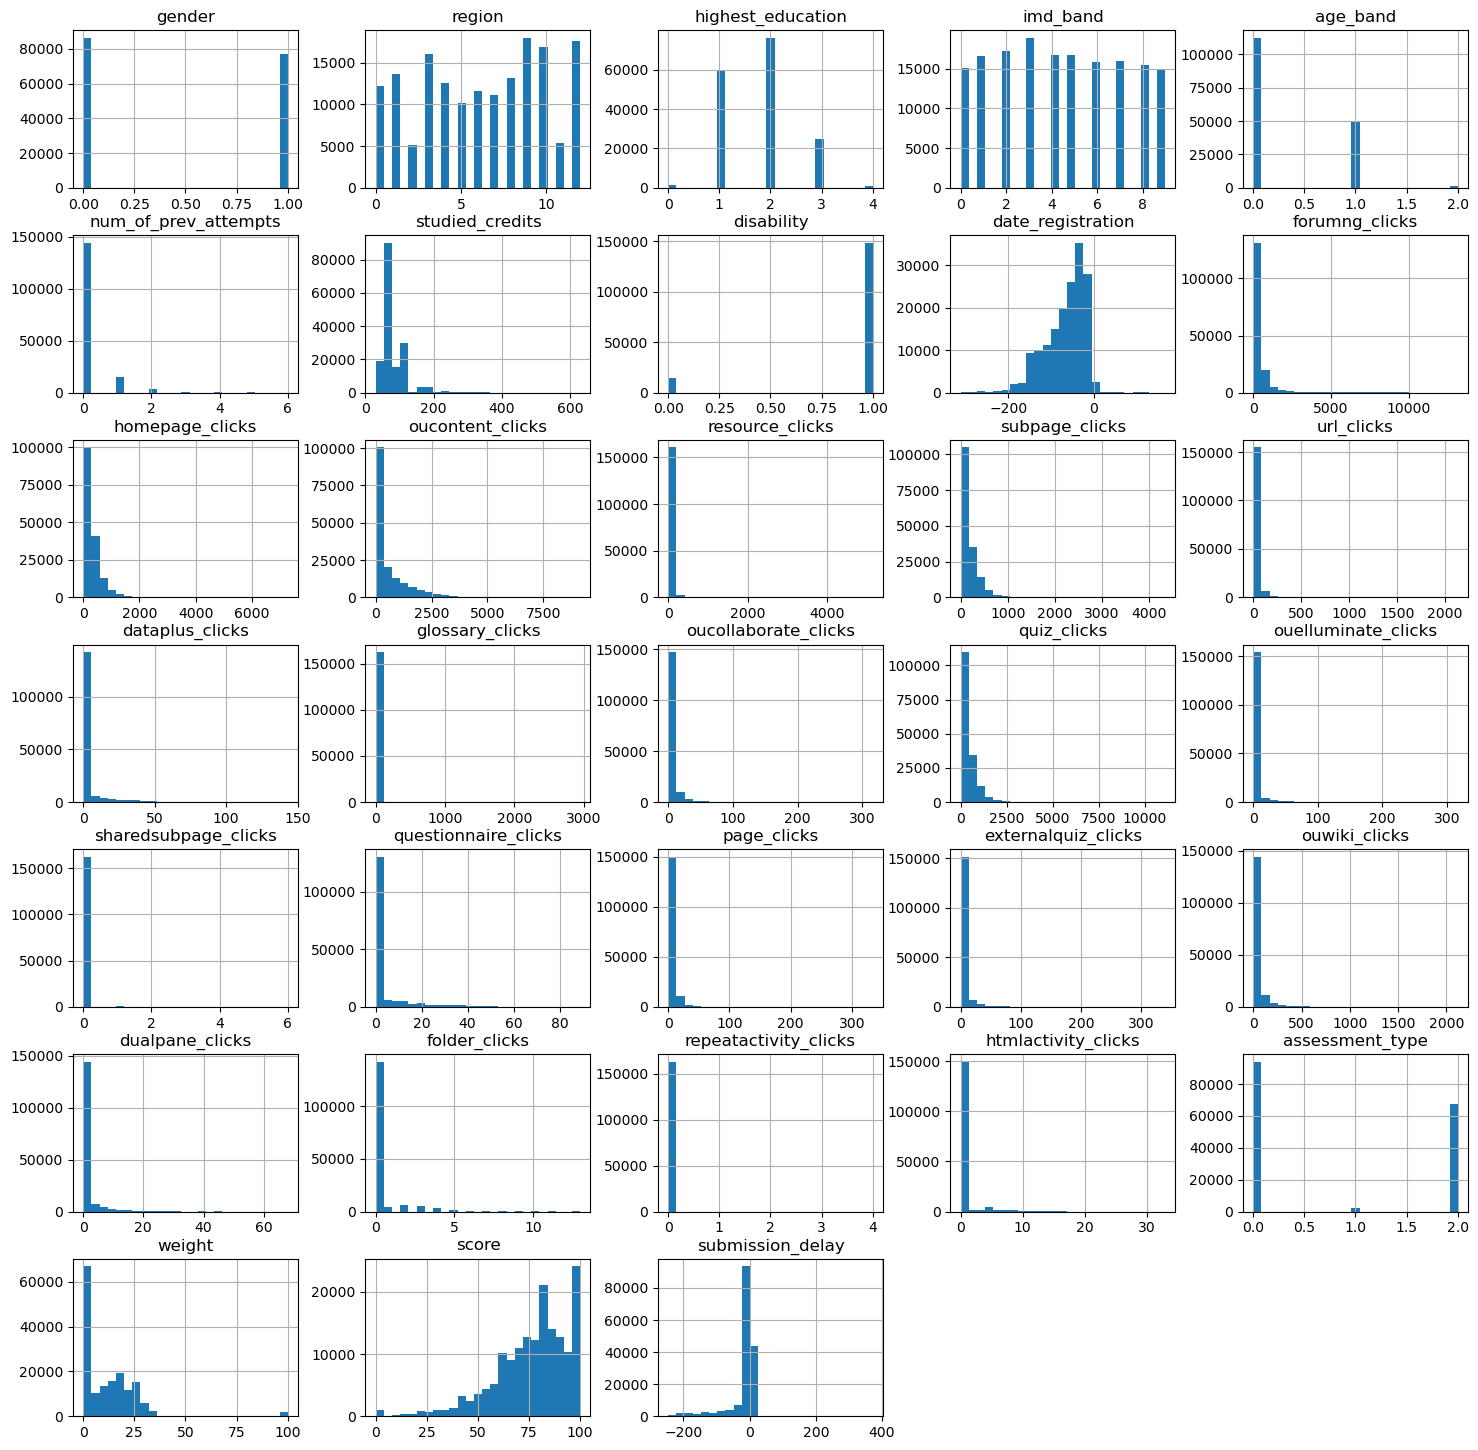
\includegraphics[width=0.7\textwidth]{data_distribution.png}
\caption{\label{fig:distr}Histograms showing the data distribution in our dataset}
\end{figure}

\subsection{Data analysis}

We computed the correlation matrix for the features of the dataset (Figure \ref{fig:corrmatr}) and observed that there exist some positive correlation between the clicks on different types of online resources (e.g. \textit{homepage clicks} and \textit{forumng clicks}, \textit{questionnaire clicks} and \textit{dataplus clicks} or \textit{oucontent clicks}), probably because they are often accessed sequentially during a single VLE session. There is also a slight negative correlation between the \textit{submission delay} and the number of clicks on some type of resources (e.g. \textit{oucontent}, \textit{quiz}, \textit{questionnaire}), suggesting that a student who is active on the VLE is more likely to submit an assignement with a small delay than a student who don't access online materials.\\

\begin{figure}[h!]
\centering
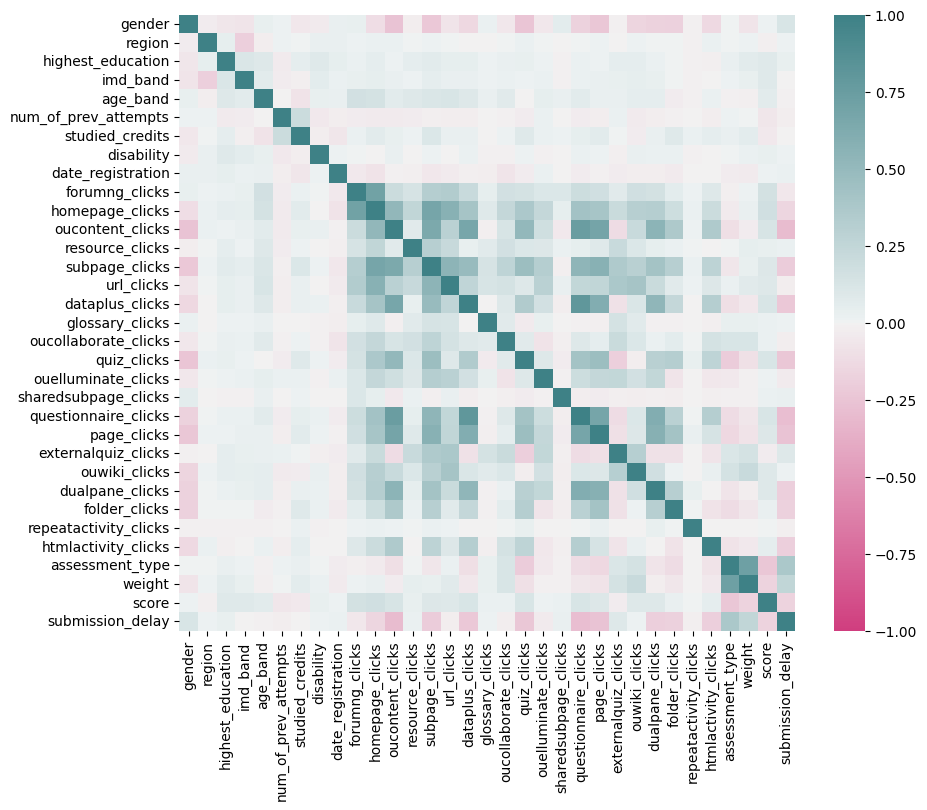
\includegraphics[width=0.8\textwidth]{correlationmatrix.png}
\caption{\label{fig:corrmatr}Correlation matrix for the dataset features}
\end{figure}

We also looked at some scatterplots expressing the relationship between each feature and the target variable (Figure \ref{fig:scatt}), noticing that in some cases the feature don't seem to influence the score value (e.g. \textit{gender}, \textit{region}, \textit{imd band}), whereas other plots show that bigger feature values are associated to larger scores (e.g. \textit{num. of prev. attempts}, \textit{forumng clicks}, \textit{questionnaire clicks}). We count on the latter type of features for the effectiveness of our linear ML models.\\
\newpage

\begin{figure}[h!]
\centering
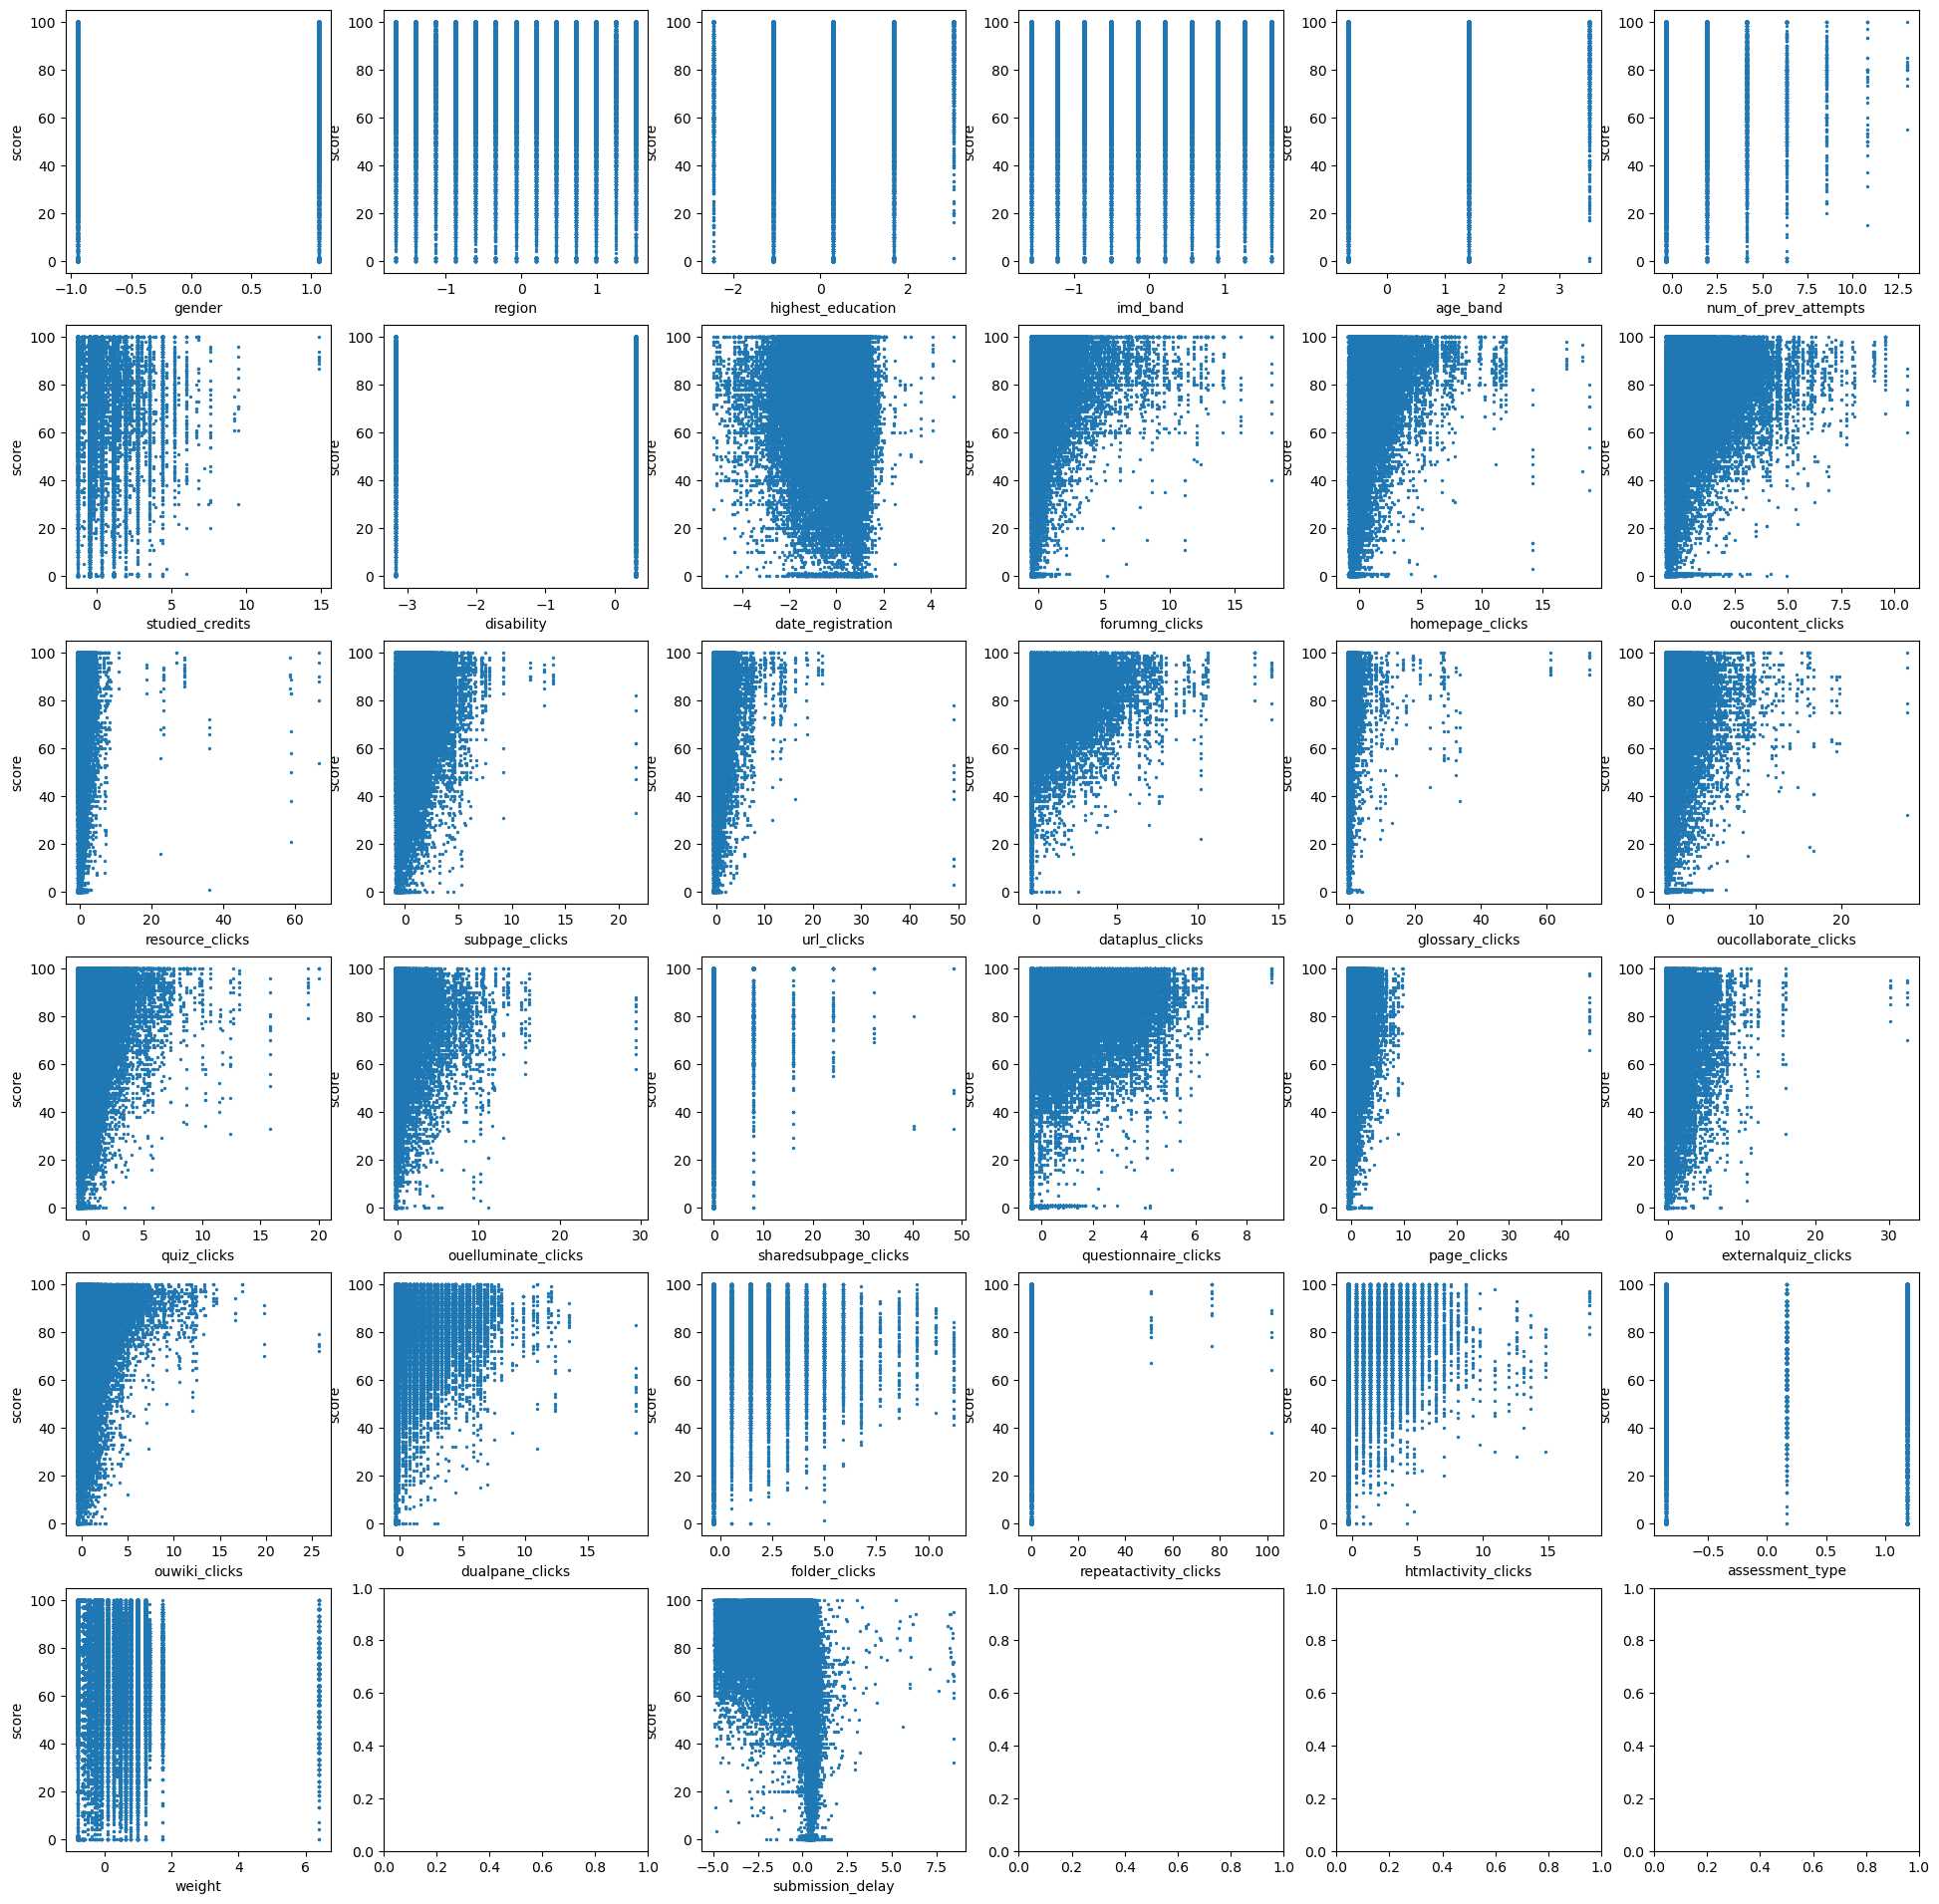
\includegraphics[width=0.43\textwidth]{scatterplots.png}
\caption{\label{fig:scatt}Scatterplots showing the relationship between each feature and the target variable}
\end{figure}

Finally, we observed that the dataset contains much more information about students who got high scores in assessments than about students with worse exam outcome (Figure \ref{fig:misrepr}). Although having many students with high grades is good news, this might interfere with the correct prediction of low scores. Detection of students at risk of failing might be of interest, so we tried to counter the problem with oversampling (Section \ref{subsec:oversamp}).

\begin{figure}[h!]
\centering
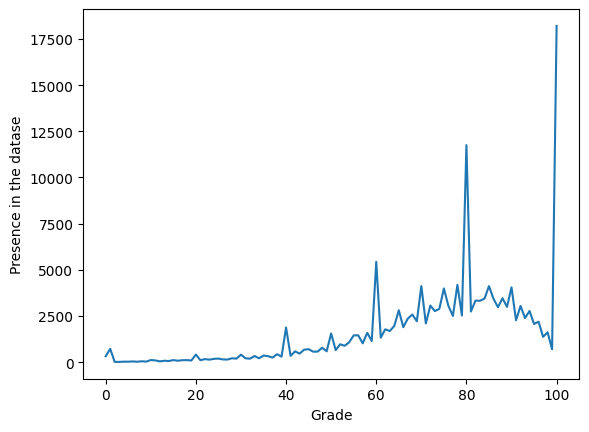
\includegraphics[width=0.6\textwidth]{misrepr.png}
\caption{\label{fig:misrepr}A graph showing the number of dataset rows for each score value}
\end{figure}

\subsection{Oversampling}
\label{subsec:oversamp}
As we discussed earlier, the training set and the dataset itselfs are heavily imbalanced (Figure \ref{fig:misrepr}), containing more \textit{higher grade} entries than \textit{lower grade} ones.
We tried solving this problem by \textit{Oversampling} the \textbf{training} data.
We used the \textit{\href{https://imbalanced-learn.org/stable/references/generated/imblearn.over_sampling.RandomOverSampler.html}{imbalanced-learn}}'s \textit{RandomOverSampler} implementation.
\begin{figure}[ht]
    \centering
    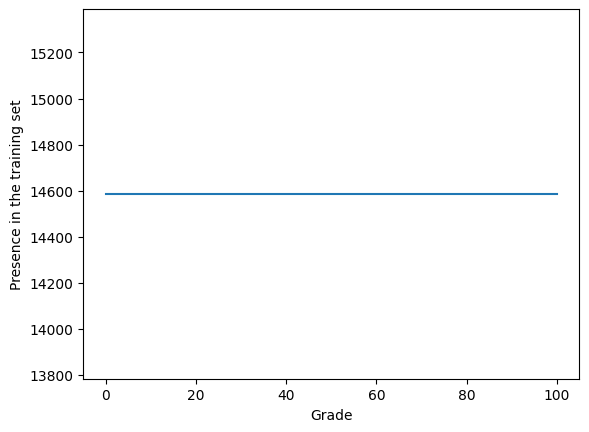
\includegraphics[width=0.6\textwidth]{dataset-presence-over.png}
    \caption{Grade presence in the training set after \textit{Oversampling}}
    \label{fig:dataset-presence-over}
\end{figure}
\newpage
This implementation randomly creates new data points, close to the existing ones, until every grade has the same 'presence' in the training set (Figure \ref{fig:dataset-presence-over}).
We tested every model both with the standard training set and the oversampled one.


\subsection{Train and test split}

We chose to compute the training and test sets for our ML models by splitting the dataset with the \textit{train\_test\_split} function from the \textit{scikit-learn} library to use 80\% of the original number of samples for training (about 130,700 rows) and the remaining 20\% for testing (about 32,600 rows).

\section{ML models training and testing}
We leveraged the \textit{scikit-learn} Python library to implement some ML models for the regression and classification tasks of predicting the score of a student in a module-presentation assessment. We trained linear (\textit{linear regression}, \textit{logistic regression}) and non-linear (\textit{decision trees}, \textit{KNN}, \textit{neural networks}) models to see if there are some differences in the results they provide.\\

We evaluated our regression models by computing the \textit{RMSE} and \textit{R2} scores, while we considered the \textit{accuracy} and the \textit{recall} for our classification models.

\subsection{Linear regression}
\FloatBarrier
Linear regression is a simple ML model. It's a linear model so there's no risk to overfit data.

We want to predict the score of a student, we use the \textit{scikit-learn LinearRegression} class (\url{https://scikit-learn.org/stable/modules/generated/sklearn.linear_model.LinearRegression.html}). It doest have any relevant hyperparameters.
We have reached a RMSE of about 17.57 and a R2 score of 0.11 on the test set and similar values on the train set since it can't overfit data.
As we can from Figure \ref{fig:errorGraph}, the model makes bigger mistakes when trying to predict lower scores (Figure \ref{fig:dtperf}), due to the big gap between the number of students with high and low scores that are present in the dataset. 

\begin{figure}[h!]
    \centering
    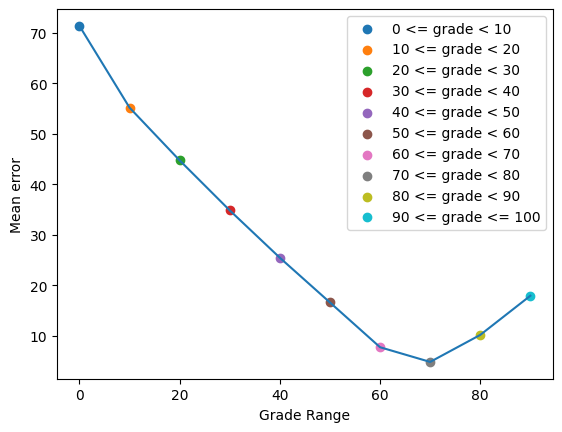
\includegraphics[width=0.6\textwidth]{grades_errors.png}
    \caption{A graph showing the mean error for 10 ranges of grades}
    \label{fig:errorGraph}
\end{figure}

\begin{figure}[h!]
    \centering
    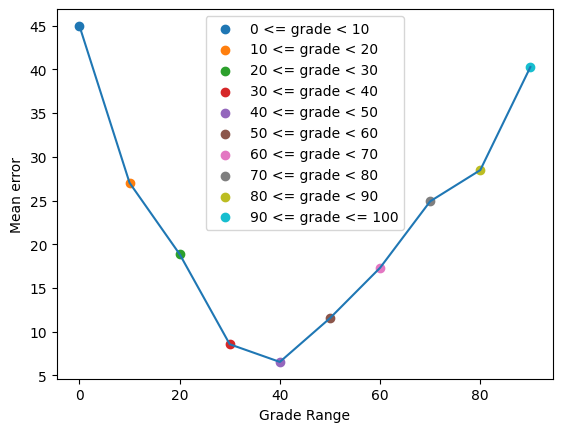
\includegraphics[width=0.6\textwidth]{grades_errors2.png}
    \caption{A graph showing the mean error for 10 ranges of grades on the oversampled set}
    \label{fig:errorGraph2}
\end{figure}
\newpage


\subsubsection{Oversampling}
Because of that we tried to do oversampling on our dataset using the sklearn function \textit{RandomOverSampler}, now we have the same amount of data for each grade. 
We got a RMSE of about 29.95 which is higher than the not oversampled version. As we can see on the Figure \ref{fig:errorGraph2} we have a better accuracy on the lower grades but a worst accuracy on the higher on the middle ones.






\FloatBarrier

\subsection{Decision Trees}

Decision trees are a simple ML model that should be able to deal with the non-linear relationship that some features show with the target variable. However, they might be prone to overfitting, as they are built by splitting the training samples according to their values for the most important features.

\subsubsection{Hyperparameter tuning}
Since we aim to predict the exact score of a student in an assessment, we use the \textit{scikit-learn} \textit{DecisionTreeRegressor} class (\url{https://scikit-learn.org/stable/modules/generated/sklearn.tree.DecisionTreeRegressor.html}). Such implementation of decision trees has many hyperparameters, but we selected \textit{min\_samples\_leaf} and \textit{min\_samples\_split} as the the most significant ones: the former determines the minimum number of samples required to be at a leaf node, the latter specifies the minimum number of samples required to split an internal node. So these parameters influence the size of the decision tree and the extent of overfitting.\\

Some hyperparameter tuning (Figure \ref{fig:heatmap}) was done to find out the values that allow to reach the best performance: with \textit{min\_sample\_leaf} set to 45 and \textit{min\_sample\_split} set to any value between 5 and 50 we can reach an RMSE score of about 16.36 and an R2 score of 0.23 on the test set. Since the scores for the prediction on the train set were $RMSE = 15.01$ and $R2 = 0.36$ the model doesn't seem to overfit too much. \\

\begin{figure}[h!]%
    \centering
    \subfloat[\centering RMSE heatmap]{{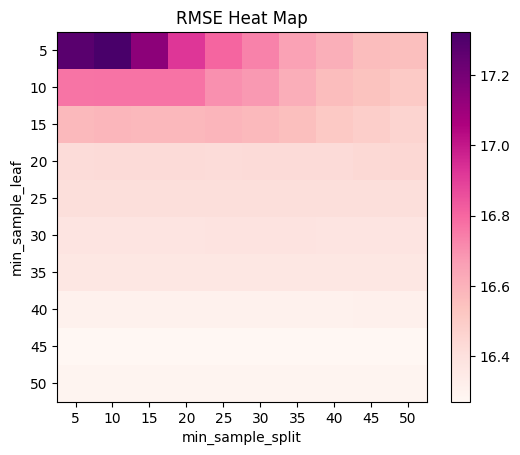
\includegraphics[width=7cm]{DTheatmap1.png} }}%
    \qquad
    \subfloat[\centering R2 score heatmap]{{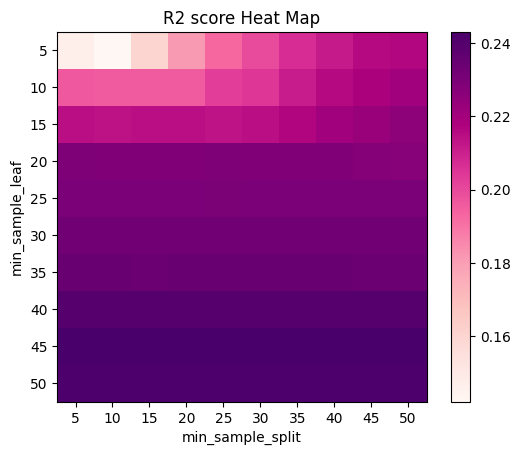
\includegraphics[width=7cm]{DTheatmap2.png} }}%
    \caption{Heatmaps showing the RMSE and R2 values for different choices of \textit{min\_sample\_leaf} and \textit{min\_sample\_split}}%
    \label{fig:heatmap}%
\end{figure}

\subsubsection{Result analysis}
By visualizing the first levels of the decision tree with the best hyperparameters values (Figure \ref{fig:dtstruct}) we understand that the features that are more relevant to the score prediction are \textit{assessment type}, \textit{homepage clicks}, \textit{weight}, \textit{submission delay}, \textit{quiz clicks}, \textit{subpage clicks}, as they are the first features chosen to split the train set on. \\

\begin{figure}[h!]
\centering
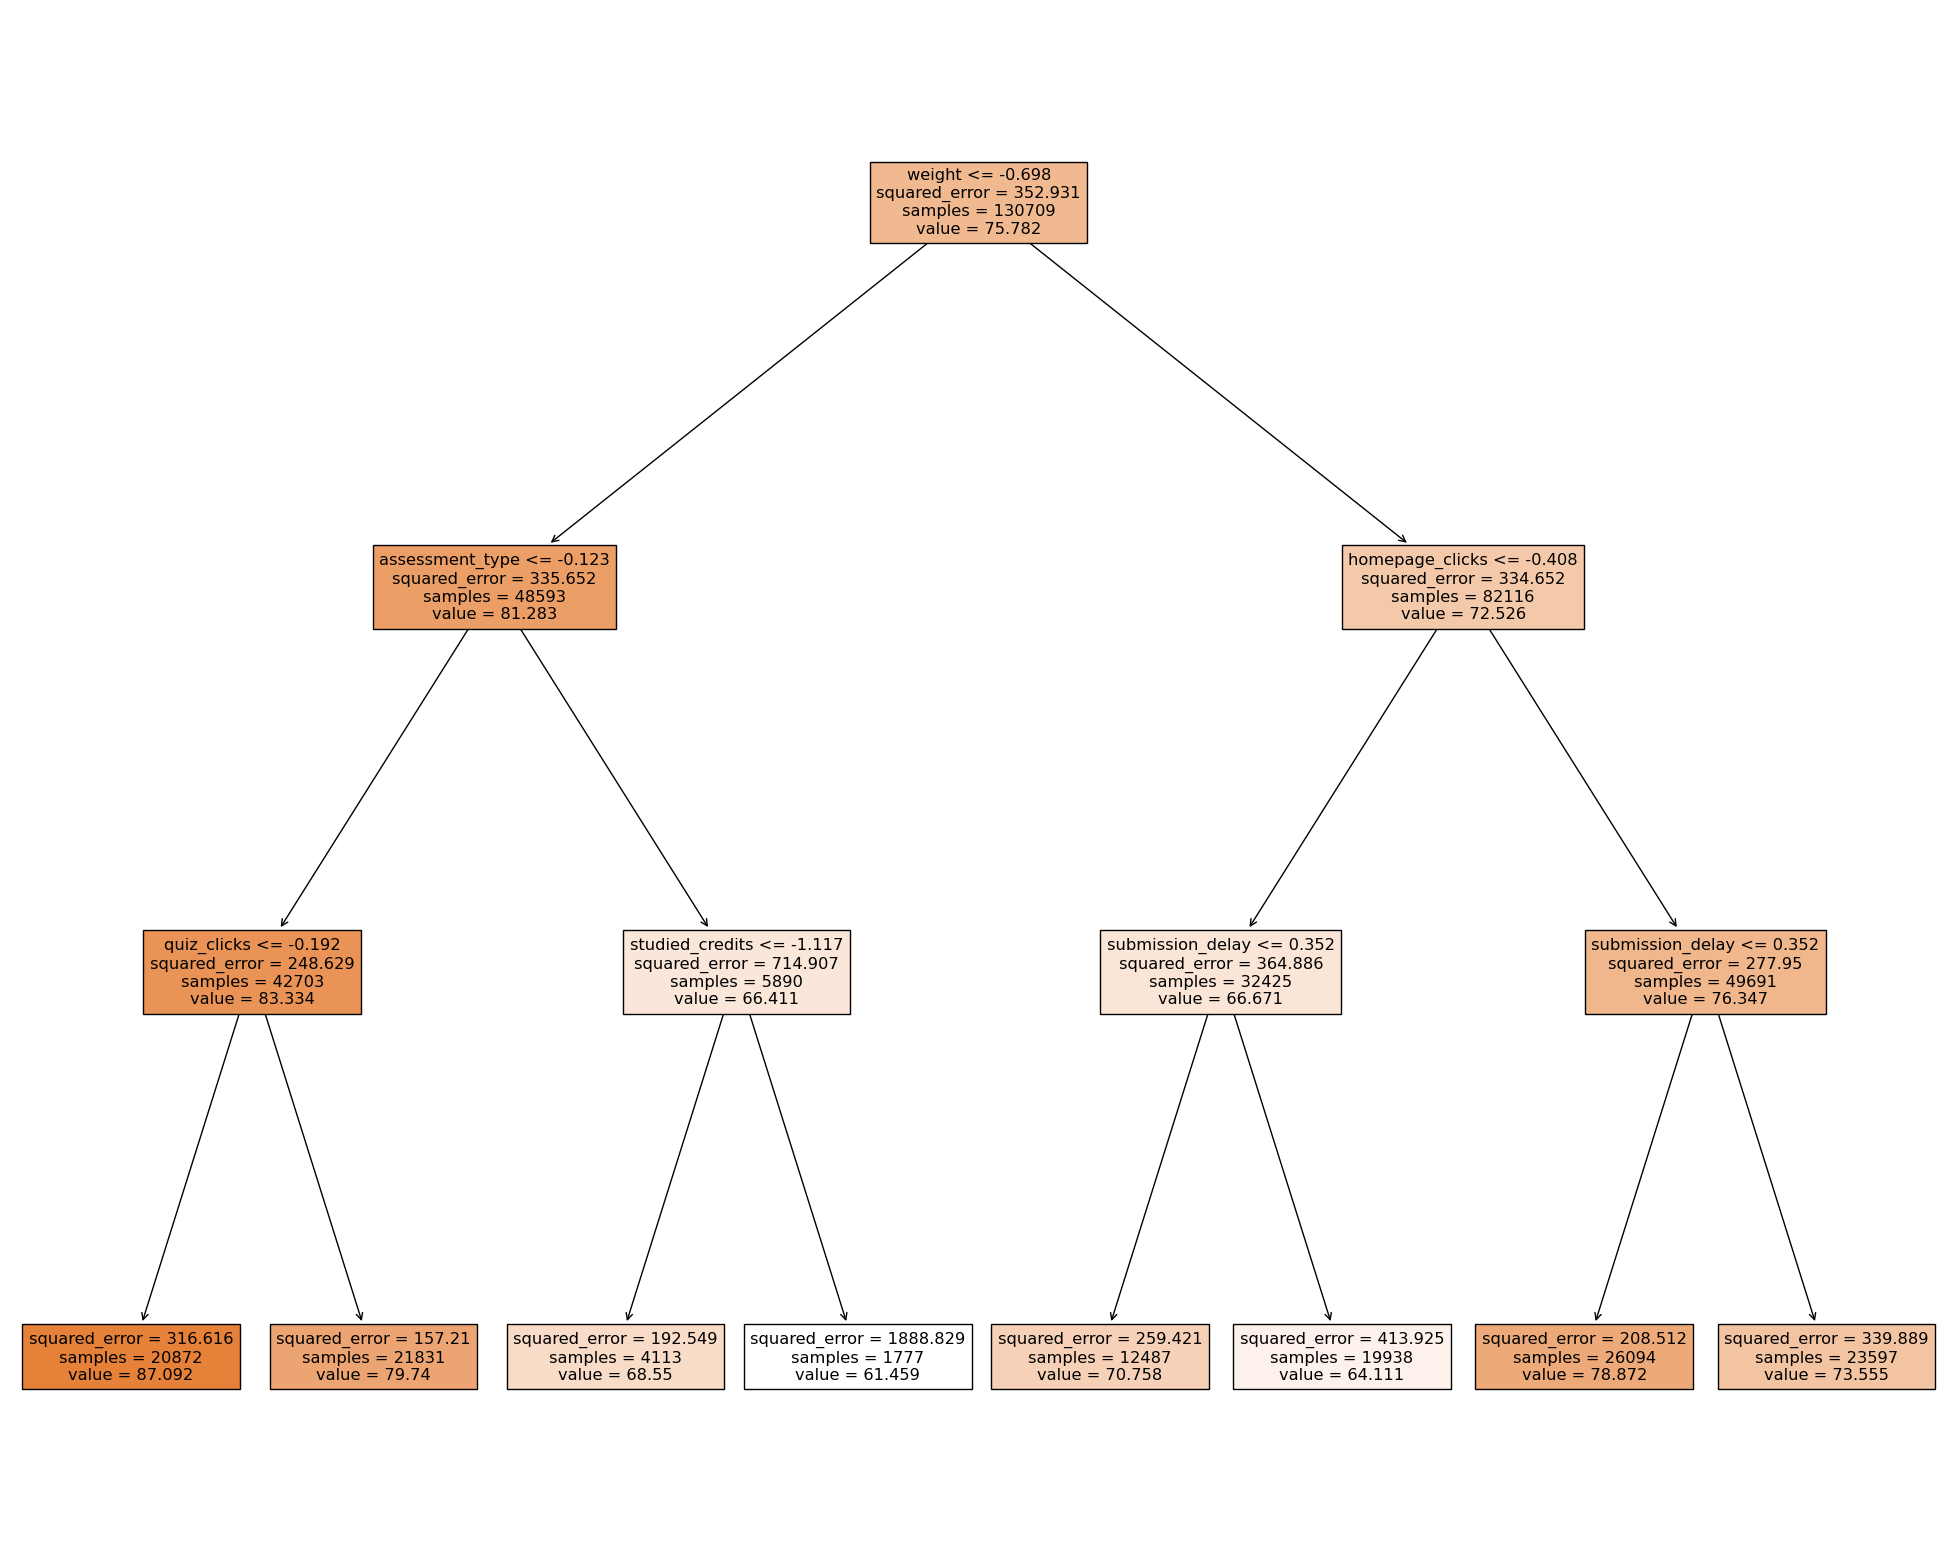
\includegraphics[width=1.0\textwidth]{DTstructure.png}
\caption{\label{fig:dtstruct}The first 4 levels of the DecisionTreeRegressor with \textit{min\_sample\_leaf} set to 45 and \textit{min\_sample\_split} set to 10}
\end{figure}
\newpage

As we expected, the model makes bigger mistakes when trying to predict lower scores (Figure \ref{fig:dtperf}): we can see that it reaches a peak of 80 points of difference from the target value when it is in the grade interval from 0 to 20, then the error starts to decrease until getting to reasonable values for target grades above 50, for which it ranges from -20 to +20. This situation is probably due to the big gap between the number of students with high and low scores that are present in the dataset. To mitigate this problem, we tried training the model on an oversampled training set (Section \ref{subsec:oversamp}).

\begin{figure}[h!]
\centering
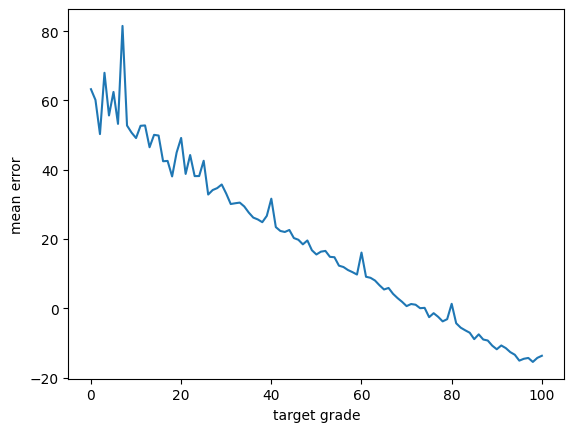
\includegraphics[width=0.5\textwidth]{DTnew.png}
\caption{\label{fig:dtperf}The mean error for each real score that the model tries to predict}
\end{figure}


\subsubsection{Oversampling}
By training the \textit{DecisionTreeRegressor} with the previously mentioned hyperparameters values on the oversampled training set obtained with \textit{Random Oversampling}, we get an \textit{RMSE score} of about 15.49 and an \textit{R2 score} of 0.31. So the performance of the model is slightly improved, with an RMSE decrease of 0.87 and an R2 increase of 0.08 compared to the results we got with the standard training set.

\begin{figure}[h!]
\centering
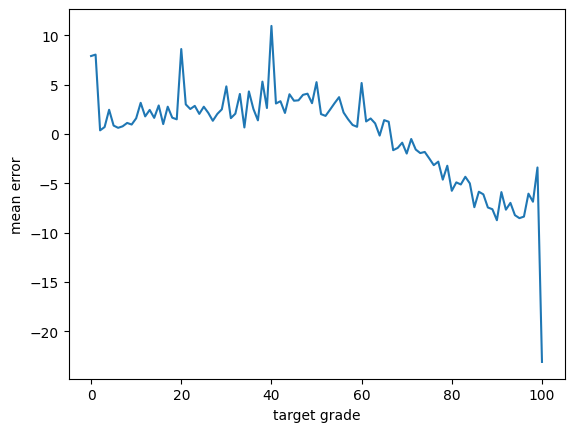
\includegraphics[width=0.5\textwidth]{DToversamp.png}
\caption{\label{fig:dtperfover}The mean error for each real score of the model trained on the oversampled set}
\end{figure}

In Figure \ref{fig:dtperfover} we see that the mean error is now almost evenly distributed across the target grades (ranging from -10 to +10), although there is a tendency of overestimating low scores and underestimating high ones, with a negative peak on the maximum score, for which an error of about -25 is registered. This situation is preferable to the one depicted in Figure \ref{fig:dtperf}, as we think it's more important to correctly detect students that are likely to get low scores, in order to provide the help they need, than precisely predicting maximum scores for students who are already well performing in their studying career.

\subsection{KNN Regression}
KNN Regression is perhaps the simplest ML model, that uses \textbf{feature similarity} to predict the values of any new data points. 
Given an input, the model returns the mean of the values corresponding to the closest $k$ points to that input.
We used the \textit{\href{https://scikit-learn.org/stable/modules/generated/sklearn.neighbors.KNeighborsClassifier.html}{scikit-learn}} implementation.

\subsubsection{Finding the best model}
In order to find the best KNN Regression model for this dataset we made predictions on different models with different $k$ values. 
We then scored every model and chose the one with the best score. The following plots (Figure \ref{fig:knn-scores}) show the \textit{RMSE} and \textit{R2} scores (y axis) for every model (x axis).
\begin{figure}[ht]
\centering
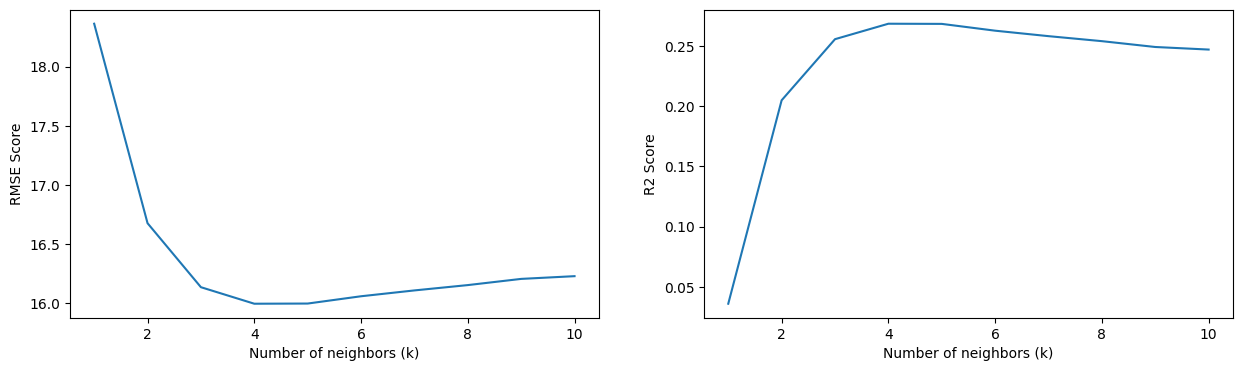
\includegraphics[width=0.95\textwidth]{KNN_scores.png}
\caption{\textit{RMSE} and \textit{R2} scores for every model}
\label{fig:knn-scores}
\end{figure}
We only analyzed models with $k = 1, \ldots, 10$.
Analyzing models with $k > 10$ would be useless, since increasing $k$ will make the model underfit the data, hence the scores will keep getting worse.
The best model for this data is the one with $k = 4$.
For this model we got a \textit{RMSE score} of around $15.9325$ and a \textit{R2 score} of around $0.2742$.
These scores are better than the previously analyzed ML models.

\subsubsection{Analyzing the results}
We want to find out if the model is better at predicting some grades than others.
\begin{figure}[ht]
\centering
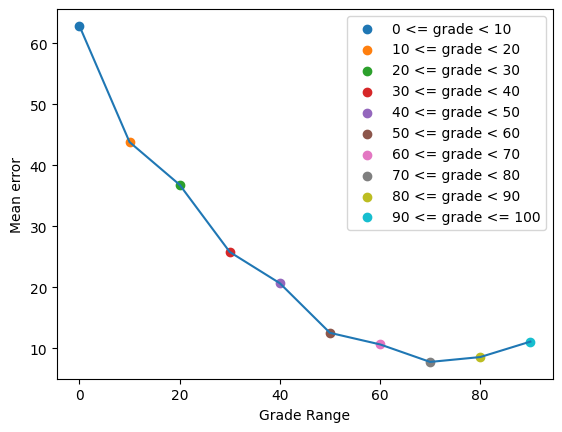
\includegraphics[width=0.5\textwidth]{KNN_errs_class.png}
\caption{Mean predictions error for grade classes}
\label{fig:knn-err}
\end{figure}
The plot in the Figure \ref{fig:knn-err} shows the mean error of the model predictions (y axis), for $10$ range of grades (x axis).
Looking at the plot it's clear that the model is better at predicting \textit{higher} grades than \textit{lower} ones.
This behaviour was expected, since the dataset is heavily imbalanced and contains few \textit{low} grades.

\subsubsection{Oversampling}
As previously mentioned we tried \textit{Random Oversampling} in order to solve the imbalance problem of the dataset.
We found the best value for $k$ with this \textit{Oversampled} dataset, just like we did in the normal one.
\begin{figure}[ht]
\centering
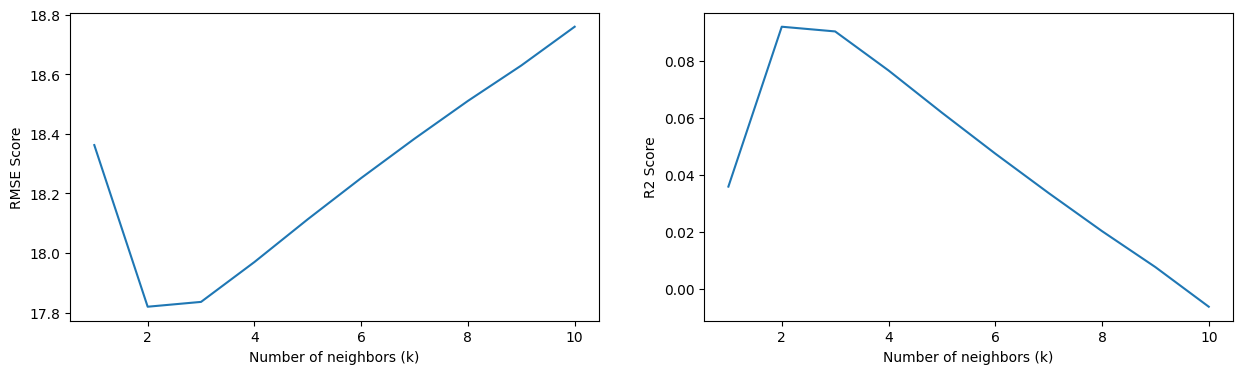
\includegraphics[width=0.95\textwidth]{KNN_scores_over.png}
\caption{\textit{RMSE} and \textit{R2} scores for every model, with \textit{Oversampled} dataset}
\label{fig:knn-scores-over}
\end{figure}
As shown in Figure \ref{fig:knn-scores-over} the best model is the one with $k = 2$.
For this model we got a \textit{RMSE score} of around $17.8199$ and a \textit{R2 score} of around $0.0921$.
\begin{figure}[ht]
\centering
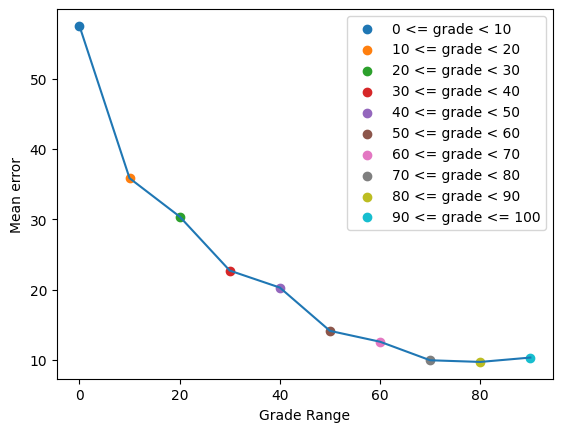
\includegraphics[width=0.5\textwidth]{KNN_errs_class_over.png}
\caption{Mean predictions error for grade classes, with \textit{Oversampled} dataset}
\label{fig:knn-err-over}
\end{figure}
These scores are worse than the ones obtained predicting with the standard dataset, but effectively this model is better at predicting \textit{lower} grades (Figure \ref{fig:knn-err-over}).

\FloatBarrier
\subsection{Logistic regression}

Logistic regression is a statistical model suited for predicting the probability of an event occurring. In our case, given an assessment $A$ and a range of grades $[a,b]$ , the event we want to predict the probability of is "$A$'s grade falls in the range $[a,b]$". 

\subsubsection{Assigning the classes}

In order to work with this model, first we have to find a way to divide the assessments in the dataset in different classes. To do this, we tried different approaches, but first, let's define the notation:
\begin{itemize}
\item[] $C$: set of the classes. If we want to divide the students in 5 classes, $C$ will be $\{1,2,3,4,5\}$

\item[] $Y$: array of target values

\item[] $Y_c[i]$: array of the classes assigned to each entry in $Y$

\end{itemize}

$Y_c$ is such that:
$$
\forall i \in \{0, 1, 2, \ldots, \text{{len(Y)}}-1\}, Y_c[i] \in C
$$
and, if $Y_c[i] = n$, it means that $Y[i]$ belongs to class $n$

Now we can define the different ways in which we can divide the dataset:

\begin{itemize}
    \item \textbf{uniform grades (UnGr)}: divide the total range of grades uniformly, so $Y_c$ is to be assigned as follows:

    $$
Y_c[i]=\left\lceil\frac{Y[i]-\min{Y}}{\frac{\max{Y}-\min{Y}}{\lvert C\rvert}}\right\rceil
$$

suppose we want 5 classes, assessments whose grade falls in the range $[0,20]$ will be assigned to class $1$, those associated to range $[20,40]$ will be assigned to class 2, and so on. 

Due to the previously highlighted underrepresentation problem, this division results in heavily imbalanced classes, with fewer examples for classes representing worse grades and more examples for other classes.

 \item \textbf{uniform classes (UnCl)} : divide the dataset such that the resulting classes will have the same number of examples.

 Let $Y_{sort}$ be the sorted version of $Y$, and let $Y_{index}$ be the array of the assigned position for each value in $Y$ in its sorted version $Y_{sort}$:
$$
(Y[i]=v \land Y_{index}[i]= j ) \Rightarrow Y_{sort}[j]=v
$$
Then, $Y_c$ is assigned as follows:
$$
Y_c[i]=\left\lceil \frac{Y_{index}[i]}{\frac{len(Y)}{\lvert C \rvert}} \right\rceil
$$

\item \textbf{uniform contribution (UnCo)}: divide the dataset such that the sum of the grades for each class's examples is the same. $Y_c$ is then assigned as follows: $$
Y_c[i]=\left\lceil \frac{\sum\limits_{j\leq i} Y_{sort}[j]}{\frac{\sum\limits_j Y[j]}{\lvert C \rvert}} \right\rceil
$$

\item \textbf{fail/pass (F/P)}: Divide the dataset in 2 classes. For each example, the assigned class reflects whether the assessment is successful (grade is above 40) or a failure (grade is lower or equal to 40).
$$
Y_c[i]= \min{[1,\left\lfloor \frac{Y[i]}{40} \right\rfloor ]} +1
$$

\end{itemize}

It is important to notice that \textbf{UnCl} and \textbf{UnCo}, while exhibiting more balanced classes, still don't solve the class imbalance problem: when they are used to assign the classes to the assessments, classes containing assessments with lower scores will span upon a quite wide range, compared to other classes (for instance, class 1 might include assessments with a grade in the range $[0-67]$, while class 5 could easily include assessments with a grade in $[95-100]$)

\subsubsection{Implementation and oversampling}

As for the implementation of the logistic regression model, we took advantage of \textit{scikit-learn}'s {\href{https://scikit-learn.org/stable/modules/generated/sklearn.linear_model.LogisticRegression.html}{LogisticRegression}} class. It allows to specify a number of parameters (\textit{penalty},\textit{class\_weight},\textit{solver},...), none of which heavily influences the results that we obtained.

By applying such model to the data as it is, we get the confusion matrices in figure \ref{fig:CMnoOS}
\begin{figure}[h!]
    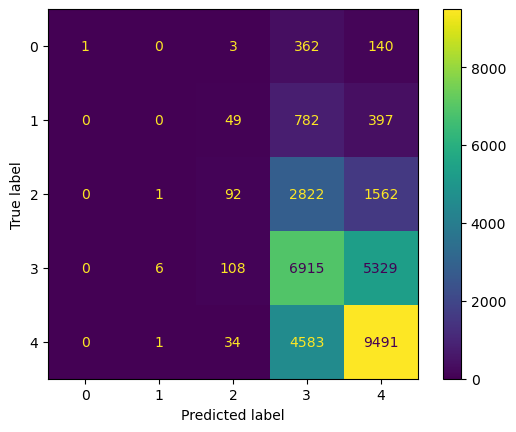
\includegraphics[width=.24\textwidth]{UnRa0.png}
    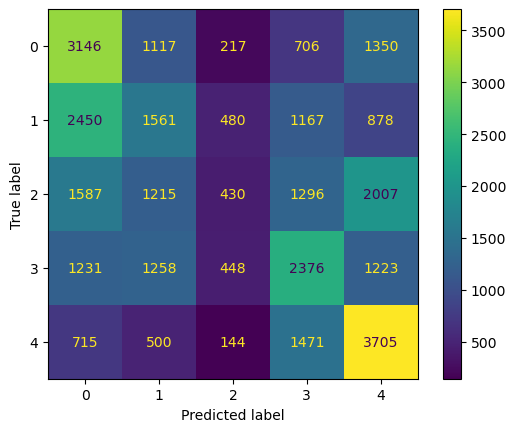
\includegraphics[width=.24\textwidth]{UnCl0.png}
    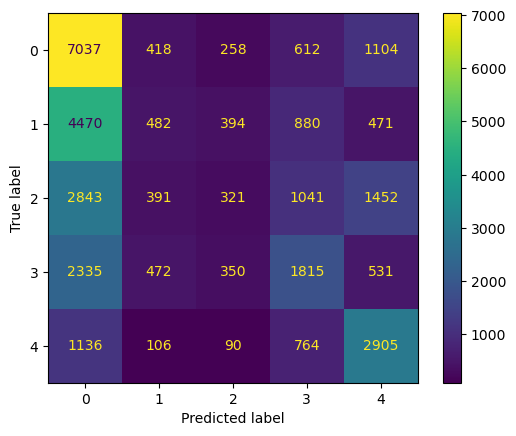
\includegraphics[width=.24\textwidth]{UnGr0.png}
    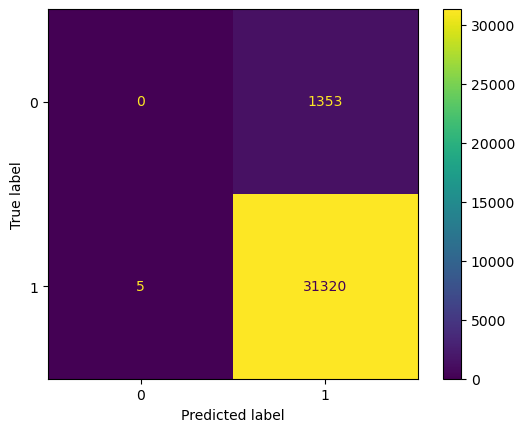
\includegraphics[width=.24\textwidth]{FP0.png}
    \caption{confusion matrices for logistic regression without oversampling. From left to right: \textit{UnGr}, \textit{UnCl}, \textit{UnCo} and \textit{F/P}. Classes go from 0 to 4 instad of going from 1 to 5 }
    \label{fig:CMnoOS}
\end{figure}

As expected, without any kind of precautionary measure on the class imbalance, we get a model that's really bad at detecting failing assessments (\textit{UnGr}, matrix on the leftmost). This is because the majority of the dataset is classified as class 3 or 4, and other classes clearly do not get enough support to influence significantly the model. The problem is even more evident when we consider the confusion matrix for \textit{F/P}, as in this case almost all of the example in the test set is classified as 1 (pass).\textit{UnCl} and \textit{UnCo} do a better job at distinguishing assessments with low grades from assessment with high grades, but they end up in polarizing their decisions: either an assessment belongs to the higher class, or to the lower class.

With the objective of mitigating the effect of the class imbalance, we execute oversampling on the dataset via the {\href{https://imbalanced-learn.org/stable/references/generated/imblearn.over_sampling.RandomOverSampler.html}{RandomOverSampler}} class from \textit{imbalanced-learn}, which naively oversamples the data by picking samples at random with replacement. Thus we get the results in figure \ref{fig:CMwOS}

\begin{figure}[h!]
    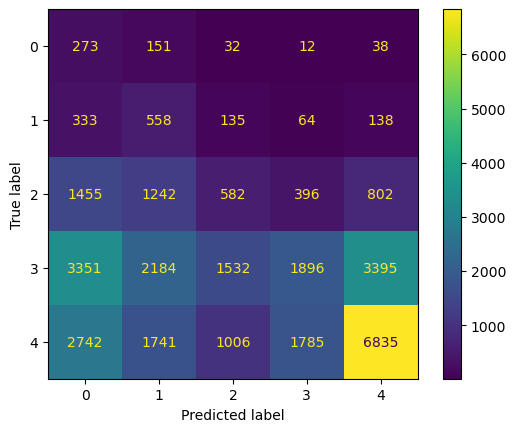
\includegraphics[width=.24\textwidth]{UnRa1.png}
    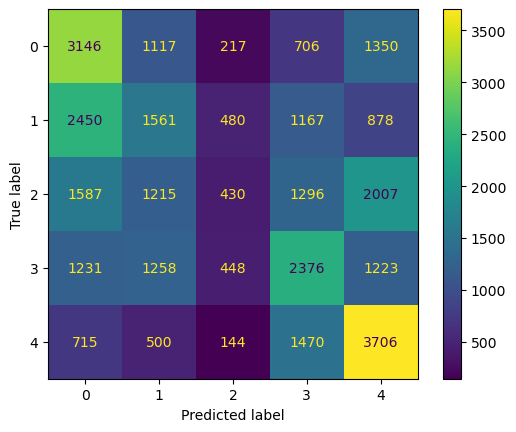
\includegraphics[width=.24\textwidth]{UnCl1.png}
    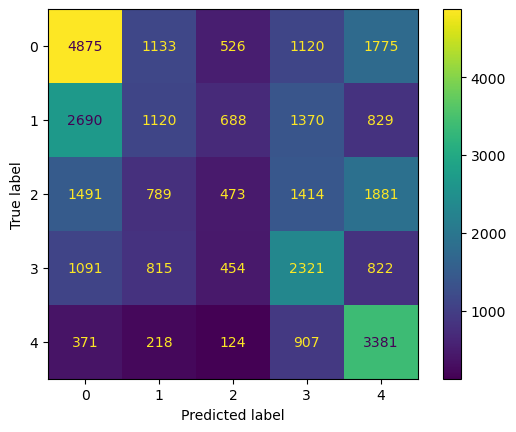
\includegraphics[width=.24\textwidth]{UnGr1.png}
    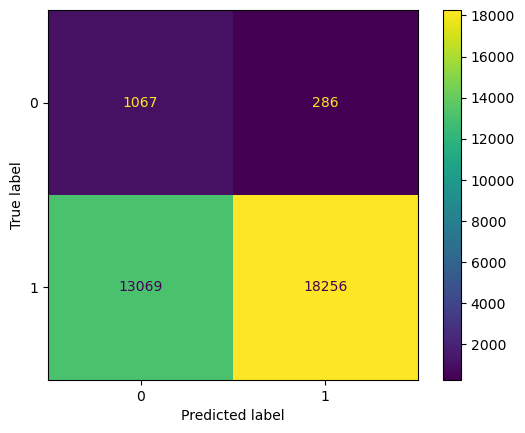
\includegraphics[width=.24\textwidth]{FP1.png}
    \caption{confusion matrices for logistic regression with naive oversampling. From left to right: \textit{UnGr}, \textit{UnCl}, \textit{UnCo} and \textit{F/P}. Classes go from 0 to 4 instad of going from 1 to 5 }
    \label{fig:CMwOS}
\end{figure}

While \textit{UnCl} and \textit{UnCo} don't seem to benefit much from oversampling, we get an interesting result from \textit{UnGr} and \textit{F/P}: even though assessments with higher grades are harder to predict, the amount of assessment with low grades that are correctly predicted increases significantly. We consider this to be a meaningful result, since detecting students that are at risk of failing an assessment and being able to support them is much more important than detecting students that are doing fine.

\subsubsection{Results}

In this section, we may observe some of the results obtained through our analysis. We evaluated the performance of logistic regression not only for the dataset as it is and on the randomly oversampled dataset, but also on a dataset oversampled via SMOTE (an oversampling technique that generates new synthetic data) and on a dataset enriched with polynomial features (thanks to \textit{scikit-learn}'s {\href{https://scikit-learn.org/stable/modules/generated/sklearn.preprocessing.PolynomialFeatures.html}{PolynomialFeatures}} class).
\begin{table}[h!]
  \centering
  \begin{tabular}{|p{3cm}|c|c|c|c|c|c|c|c|c|c|c|c|c|}
    \hline
     & \multicolumn{2}{|c|}{\textbf{class 0}} & \multicolumn{2}{|c|}{\textbf{class 1}} & \multicolumn{2}{|c|}{\textbf{class 2}} & \multicolumn{2}{|c|}{\textbf{class 3}} & \multicolumn{2}{|c|}{\textbf{class 4}} & \textbf{Accuracy} \\
    \hline
    & P & R & P & R & P & R & P & R & P & R &  \\
    \hline
    \textbf{UnGr no oversampling} & 1.00 & 0.00 & 0.00 & 0.00 & 0.32 & 0.02 & 0.45 & 0.56 & 0.56 & 0.67 & 0.50 \\
    \hline
    \textbf{UnGr random oversampling} & 0.03 & 0.54 & 0.09 & 0.45 & 0.18 & 0.13 & 0.46 & 0.15 & 0.61 & 0.48 & 0.31 \\
    \hline
    \textbf{UnGr SMOTE} & 0.04 & 0.56 & 0.09 & 0.45 & 0.17 & 0.13 & 0.46 & 0.16 & 0.61 & 0.49 & 0.32 \\
    \hline
    \textbf{UnGr polynomial} & 0.37 & 0.07 & 0.18 & 0.01 & 0.27 & 0.02 & 0.47 & 0.58 & 0.58 & 0.69 & 0.52 \\
    \hline
    \textbf{UnGr polynomial SMOTE} & 0.05 & 0.52 & 0.09 & 0.45 & 0.20 & 0.17 & 0.50 & 0.27 & 0.64 & 0.50 & 0.37 \\
    \hline
    \textbf{UnCl no oversampling} & 0.34 & 0.48 & 0.28 & 0.24 & 0.25 & 0.07 & 0.34 & 0.36 & 0.40 & 0.57 & 0.34 \\
    \hline
    \textbf{UnCl random oversampling} & 0.34 & 0.48 & 0.28 & 0.24 & 0.25 & 0.07 & 0.34 & 0.36 & 0.40 & 0.57 & 0.34 \\
    \hline
    \textbf{UnCl SMOTE} & 0.34 & 0.48 & 0.28 & 0.24 & 0.25 & 0.07 & 0.34 & 0.36 & 0.40 & 0.57 & 0.34 \\
    \hline
    \textbf{UnCl polynomial} & 0.38 & 0.46 & 0.31 & 0.36 & 0.26 & 0.05 & 0.35 & 0.44 & 0.49 & 0.57 & 0.38 \\
    \hline
    \textbf{UnCl polynomial SMOTE} & 0.38 & 0.46 & 0.31 & 0.36 & 0.26 & 0.05 & 0.35 & 0.44 & 0.49 & 0.57 & 0.38 \\
    \hline
    \textbf{UnCo no oversampling} & 0.39 & 0.75 & 0.26 & 0.07 & 0.23 & 0.05 & 0.36 & 0.33 & 0.45 & 0.58 & 0.38 \\
    \hline
    \textbf{UnCo random oversampling} & 0.46 & 0.52 & 0.27 & 0.17 & 0.21 & 0.08 & 0.33 & 0.42 & 0.39 & 0.68 & 0.37 \\
    \hline
    \textbf{UnCo SMOTE} & 0.46 & 0.51 & 0.27 & 0.17 & 0.21 & 0.08 & 0.32 & 0.42 & 0.39 & 0.68 & 0.37 \\
    \hline
    \textbf{UnCo polynomial} & 0.43 & 0.71 & 0.31 & 0.19 & 0.24 & 0.05 & 0.36 & 0.38 & 0.53 & 0.62 & 0.41 \\
    \hline
    \textbf{UnCo polynomial SMOTE} & 0.50 & 0.51 & 0.31 & 0.31 & 0.23 & 0.06 & 0.33 & 0.48 & 0.49 & 0.67 & 0.40 \\
    \hline
  \end{tabular}
  \caption{Evaluation metrics for multinomial case. P = precision, R = recall}
  \label{tab:EvMetMultireg}
\end{table}

\begin{table}[h!]
  \centering
  \begin{tabular}{|p{3cm}|c|c|c|c|c|}
    \hline
      & \multicolumn{2}{|c|}{\textbf{fail}} & \multicolumn{2}{|c|}{\textbf{pass}} & \textbf{Accuracy} \\
    \hline
    & P & R & P & R &  \\
    \hline
    \textbf{P/F no oversampling} & 0.00 & 0.00 & 0.96 & 1.00 & 0.96 \\
    \hline
    \textbf{P/F random oversampling} & 0.08 & 0.79 & 0.98 & 0.58 & 0.59 \\
    \hline
    \textbf{P/F SMOTE} & 0.08 & 0.78 & 0.98 & 0.59 & 0.60 \\
    \hline
    \textbf{P/F polynomial} & 0.25 & 0.01 & 0.96 & 1.00 & 0.96 \\
    \hline
    \textbf{P/F polynomial SMOTE} & 0.10 & 0.78 & 0.99 & 0.69 & 0.69 \\
    \hline
  \end{tabular}
  \caption{Evaluation metrics for binomial case. P = precision, R = recall}
  \label{tab:EvMetBinreg}
\end{table}

\FloatBarrier
\subsection{Neural Networks}
\FloatBarrier

Neural networks are one of the most complex models in this report.
The first thing that we did was to choose a good network topology, and for this reason we tried with many different layers.

We found that the network physical composition wasn't this important for the predictions, since each of the attempts produced more or less the same 
result, so, to mantain things at a simple and manageable state, we opt for a very simple network, with just two layers and an actiavtion function 
(ReLU) in between.

The first layer had the numbers of features in input, and in output it had the same number multiplied by two. The last layer had the duty
to predict the number of classes, so either ten or two in our experiments.

\begin{figure}[h!]
    \centering
    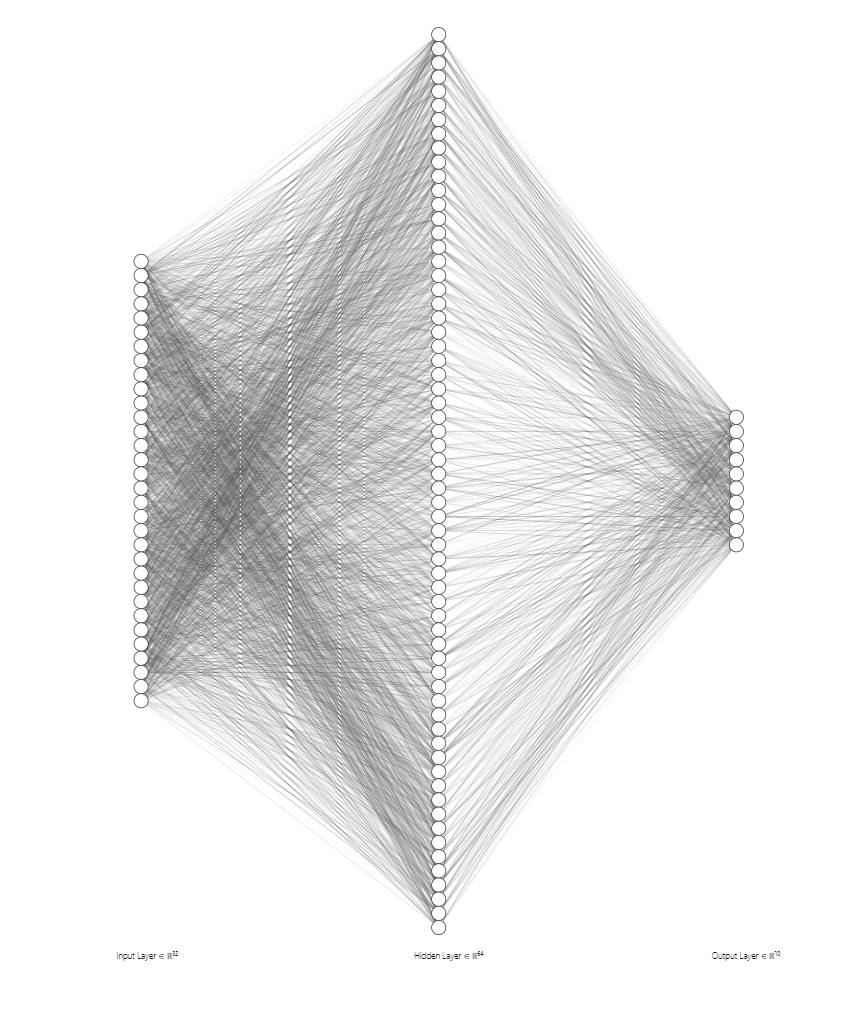
\includegraphics[width=0.5\textwidth]{nn_architecture.png}
    \caption{\label{fig:nn}The neural network architecture we used.}
\end{figure}

Since we want to predict, given the features of a student, the probability that he is gonna fall in the ranges of score we have defined, outside the last layer there is a \emph{Softmax function}, which is in charge
of parsing the outputs in probabilities. 
Understood what we said until this point, it's obvious that the loss function could not be anything other than a \emph{Cross-Entopy}.

Regarding the training, it was done using the following hyperparameters:

\begin{itemize}
    \item Defined our custom dataset, we used a \textbf{batch size} of 16.
    \item We choose a maximum of \textbf{100 epochs}, even if we didn't ever reached the limit in the training as we are gonna explain later on.
    \item We tried different \textbf{learning rates}, ranging from $10^{-1}$ to $10^{-5}$.
\end{itemize}

The training was done with the idea of stopping it when the loss was less than $5 \times 10^{-5}$. It can be clearly seen from the following graphs, that the training was almost every time stopped earlier,
especially for the smallest learning rates, that made the network change a very little for each epoch.

\begin{figure}[h!]
    \centering
    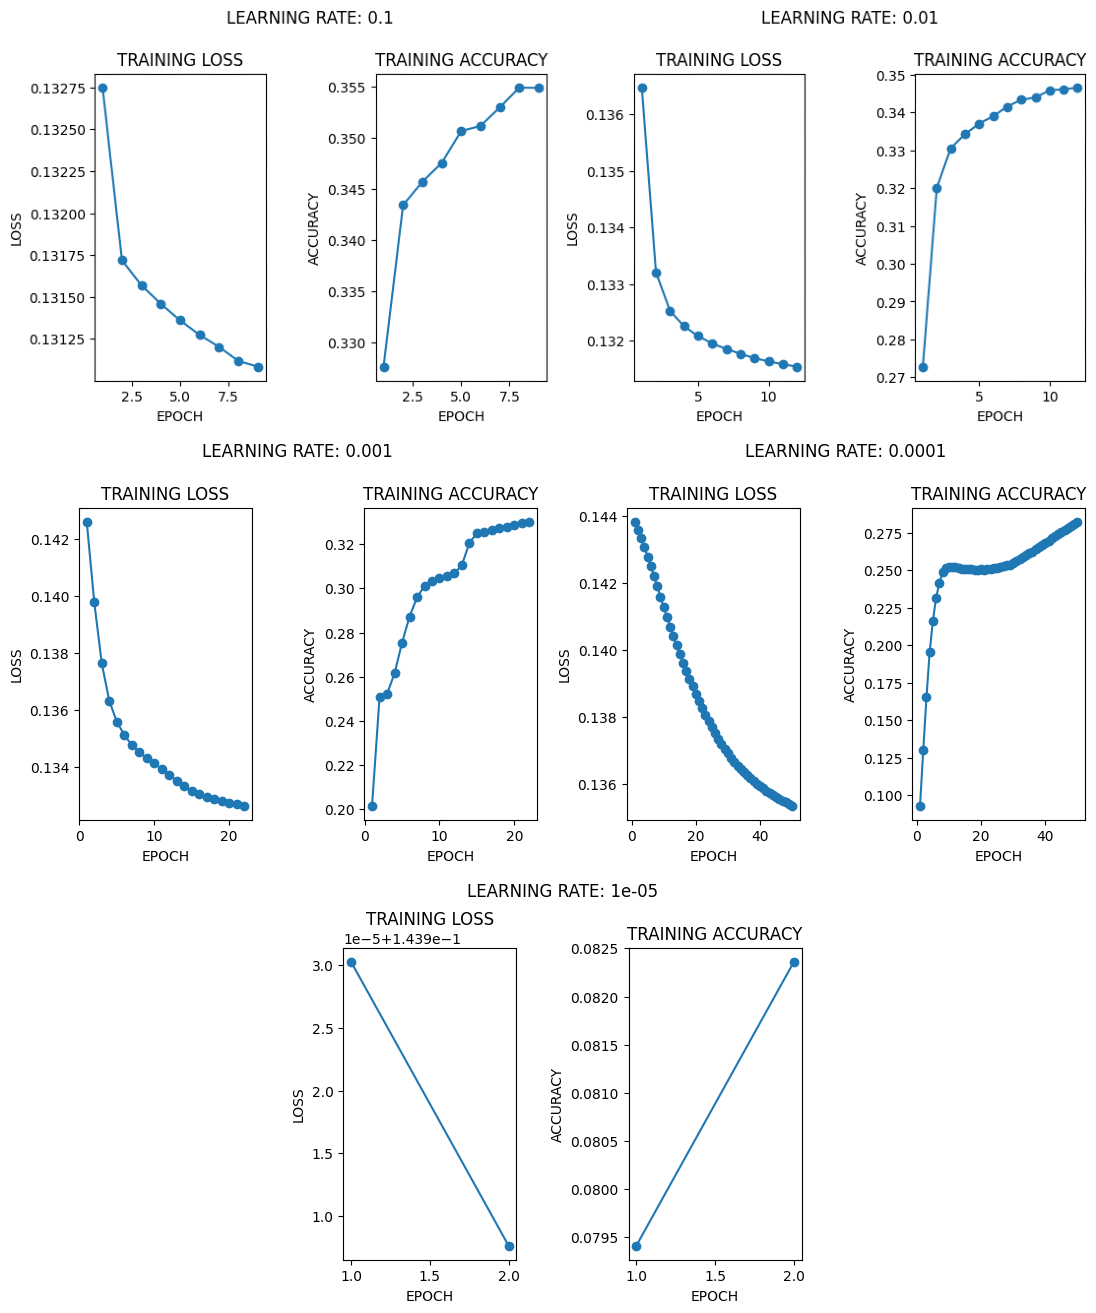
\includegraphics[width=0.5\textwidth]{lr_training.png}
    \caption{\label{fig:lr}The training we did with the different learning rates.}
\end{figure}

To provide a summary about what we said until now, we can look at the following graph, that represent the accuracy of the various models trained 
with the different learning rates on the test set:

\begin{figure}[h!]
    \centering
    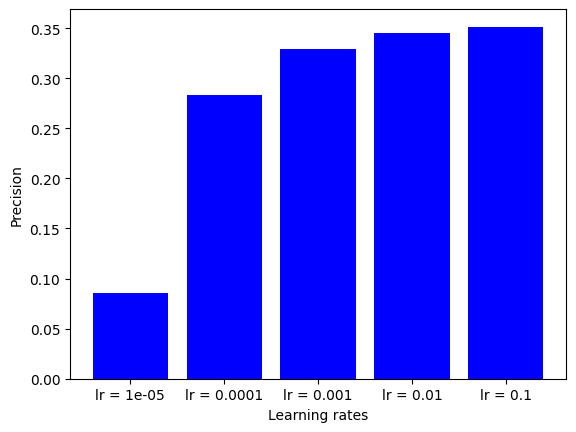
\includegraphics[width=0.5\textwidth]{results.png}
    \caption{\label{fig:summary}Summary about precisions.}
\end{figure}

The dataset chosen was afflicted by a misrepresentation problem, with more student obtaining good results and less with lower scores. For this motivation, we tried to narrow down the number of classes,
trying with just two, so higher than forty or lower.

We also changed the structure of the network, replacing the Softmax with a \emph{Sigmoid function}.

Here we can look at the results:

\begin{figure}[h!]
    \centering
    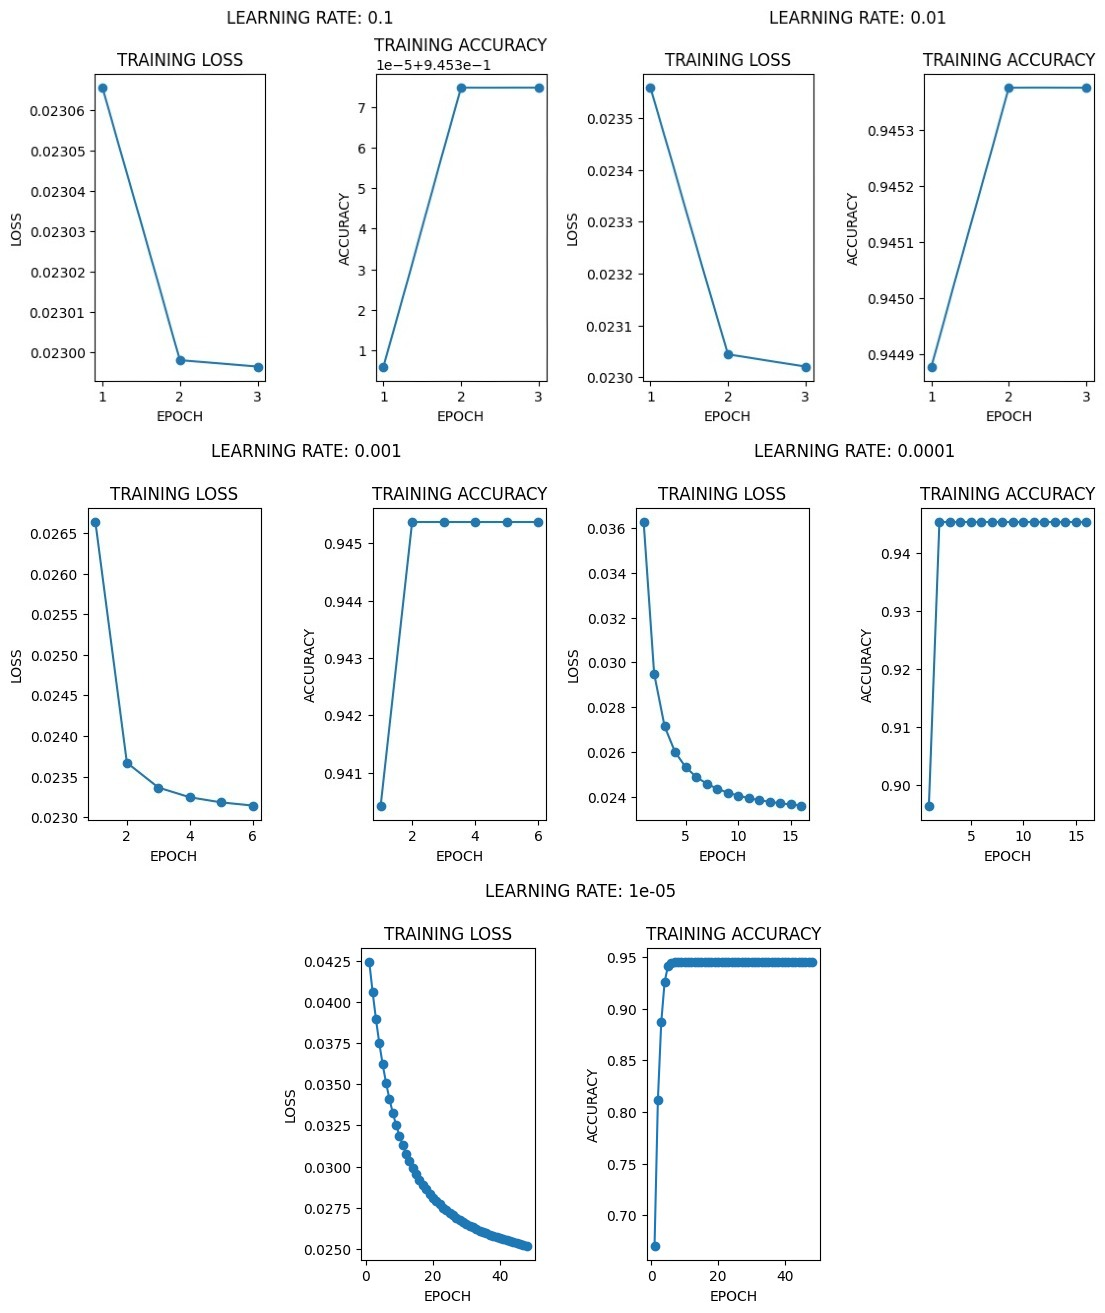
\includegraphics[width=0.5\textwidth]{binary_lr.jpg}
    \caption{\label{fig:binary_lr}Training with different learning rates with binary classification}
\end{figure}

And here we can see the following graph providing a summary on the results obtained on the test set. The misrepresentation problem appears again, 
for this motivation, the network just has to predict a value closer to one, rather than learning from the features, since a lots of examples in the dataset
are higher than forty.

\begin{figure}[h!]
    \centering
    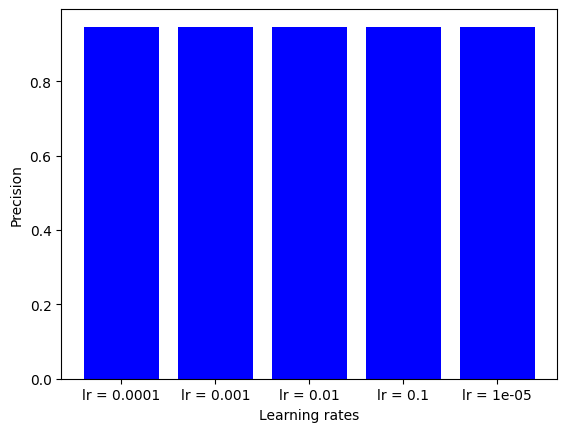
\includegraphics[width=0.5\textwidth]{binary_results.png}
    \caption{\label{fig:binary_summary}Summary of the results in binary classification.}
\end{figure}

\subsubsection{Oversampling}

As it was said before in this report and in this section, the dataset was afflicted by a misrepresentation problem. Done the oversampling, we 
tried to run again our models on the new created dataset.

In this case, the hyperparameters remained the same and we just changed the \emph{batch size} to 64, since the dataset was larger and a value
too small would have taken a lot of time for completing the training.

For the classification with ten classes we obtained:

\begin{figure}[h!]
    \centering
    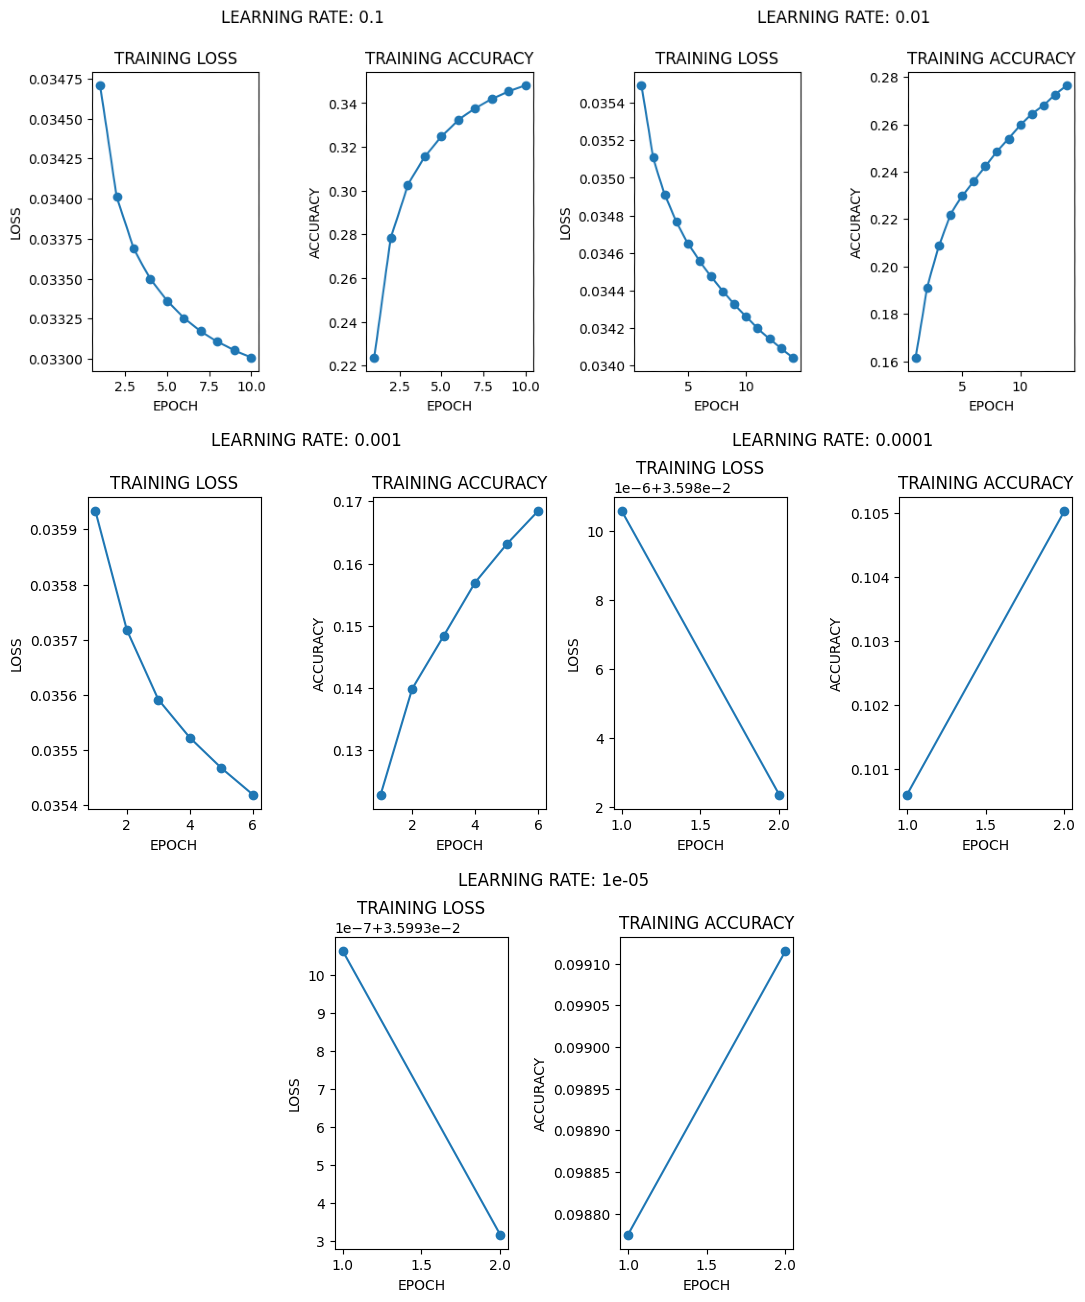
\includegraphics[width=0.5\textwidth]{nn_oversampling.png}
    \caption{\label{fig:train_oversampling}Training with oversampling.}
\end{figure}

And regarding the precision on the test dataset we had:

\begin{figure}[h!]
    \centering
    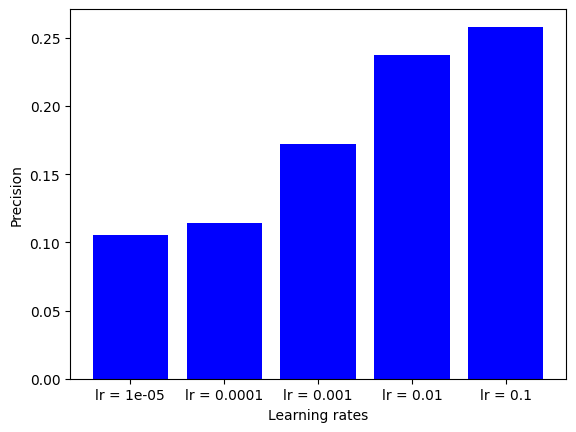
\includegraphics[width=0.5\textwidth]{precision_oversampling_nn.png}
    \caption{\label{fig:acc_oversampling}Accuracy on test dataset with training done using oversampled data}
\end{figure}

We can see that the accuracy doesn't get any higher even with oversampling. It could be speculated that the oversampling on the training data
do not solve the problem of misrepresentation in the test set, and for this motivation, the network cannot perform very well.

In the case of binary classification, now that the problem is not trivial, we can look at those new results. Since the problem got slighly more complex,
the accuracies all decreased, both for the training and for the testing:

\begin{figure}[h!]
    \centering
    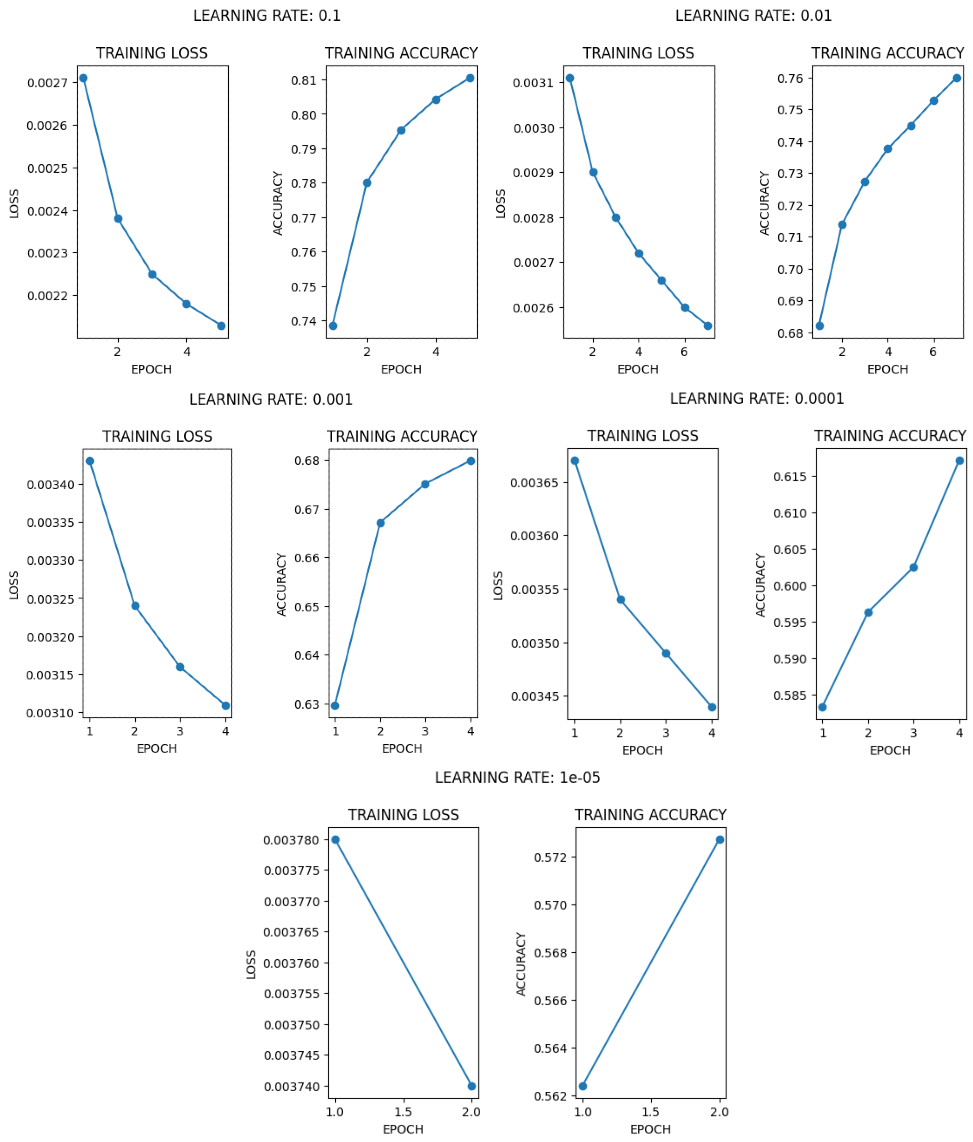
\includegraphics[width=0.5\textwidth]{binary_nn_oversampling.png}
    \caption{\label{fig:binary_train_oversampling}Training with oversampling and 2 classes.}
\end{figure}

\begin{figure}[h!]
    \centering
    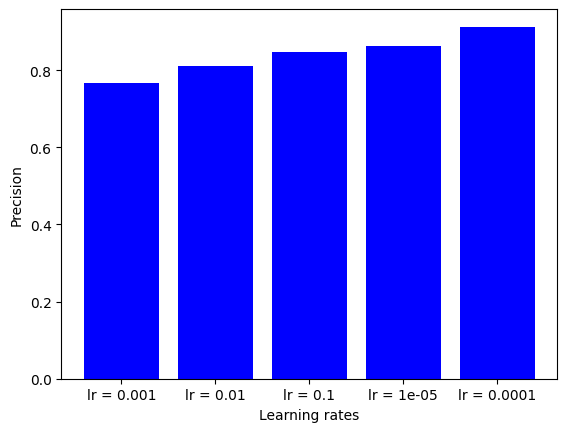
\includegraphics[width=0.5\textwidth]{precision_binary_oversampling_nn.png}
    \caption{\label{fig:binary_precision_oversampling}Precision with oversampling and 2 classes on test set.}
\end{figure}
\newpage


\section{Results analysis}
To give a final comprehensive view on what we did and discussed in this report, we provide the following tables with the results for each ML model an technique used:

\subsection{Without oversampling}

\begin{table}[h!]
    \centering
    \begin{tabular}{l|l|l|}
    \cline{2-3}
                                            & RMSE  & R2   \\ \hline
    \multicolumn{1}{|l|}{Linear Regression} & 17.57 & 0.11 \\ \hline
    \multicolumn{1}{|l|}{Decision Trees}    & 16.36 & 0.23 \\ \hline
    \multicolumn{1}{|l|}{KNN}               & 15.93 & 0.27 \\ \hline
\end{tabular}
\end{table}

\begin{table}[h!]
    \centering
    \begin{tabular}{l|l|l|l|}
    \cline{2-4}
                                              & Accuracy (10 classes) & Accuracy (5 classes)  & Accuracy (2 classes) \\ \hline
    \multicolumn{1}{|l|}{Logistic Regression} & ---                   & 0.50                  & 0.96                 \\ \hline
    \multicolumn{1}{|l|}{Neural Networks}     & 0.353                 & ----                  & 0.95                 \\ \hline
\end{tabular}
\end{table}

\subsection{With oversampling}

\begin{table}[h!]
    \centering
    \begin{tabular}{l|l|l|}
    \cline{2-3}
                                            & RMSE  & R2   \\ \hline
    \multicolumn{1}{|l|}{Linear Regression} & 29.95 & ---  \\ \hline
    \multicolumn{1}{|l|}{Decision Trees}    & 15.49 & 0.31 \\ \hline
    \multicolumn{1}{|l|}{KNN}               & 17.82 & 0.09 \\ \hline
\end{tabular}
\end{table}

\begin{table}[h!]
    \centering
    \begin{tabular}{l|l|l|l|}
    \cline{2-4}
                                              & Accuracy (10 classes) & Accuracy (5 classes)  & Accuracy (2 classes) \\ \hline
    \multicolumn{1}{|l|}{Logistic Regression} & ---                   & 0.37                  & 0.69                \\ \hline
    \multicolumn{1}{|l|}{Neural Networks}     & 0.25                  & ---                   & 0.91                \\ \hline
\end{tabular}
\end{table}



\section{Roles of team members}
We worked together on the dataset choice, data preprocessing and analysis, then each of us focused on a different ML model: 
\begin{itemize}
    \item Paolo Cursi: Linear Regression
    \item Arianna Paolini: Decision Trees
    \item Pietro Signorino: KNN Regression
    \item Tommaso Leonardi: Logistic Regression
    \item Stefano Saravalle: Neural Networks
\end{itemize}
Finally, we compared our results and discussed about them to understand what we learnt from this project.

\bibliographystyle{alpha}
\bibliography{sample}

\end{document}

